%% ===========================================================================
%%  main.tex  ·  绝对时空坐标系：音乐事件的精确量化与全局定位
%% ---------------------------------------------------------------------------
%%  学术版式（musepaper.sty）。体例：中文期刊投稿（与论文一统一）。
%%
%%  素材来源：
%%    · 开发日志/开发日志.txt                      （理论推导与叙事）
%%    · 开发日志/Muse_Agent：a profesional...md    （第一天～第八天）
%%    · 开发日志/绝对Tick_变拍号补丁_v1.md         （变拍号通式与性质说明）
%%    · 专利申请文件/最终稿件/说明书_终检版.txt     （MATCS 正式技术方案）
%%
%%  编译：双击 compile.bat ，或 xelatex 连跑三遍。
%% ===========================================================================
\documentclass[11pt,a4paper,fontset=none]{ctexart}

%% 共享字体目录（必须在 musepaper 之前声明）
\providecommand{\museFontPath}{../fonts/}
\usepackage{musepaper}
\graphicspath{{figures/}}

%% 页眉（中文期刊体例：居中排题名）
\页眉{绝对时空坐标系：音乐事件的精确量化与全局定位}

\title{绝对时空坐标系：音乐事件的精确量化与全局定位}
\author{MOZUN}
\date{}

% ===========================================================================
%% ---------------------------------------------------------------------------
%%  引用体例说明（《中央音乐学院学报》著录规范）：
%%    本刊所引文献统一以页下脚注体现，文后不再附录参考文献。
%%    故原 \begin{thebibliography} 已改为各处 \footnote。
%%    ⚠️ 规范要求著录「所引页码」；凡标【待核】/【X】处请按所据版本补齐。
%% ---------------------------------------------------------------------------
\begin{document}

% 题名页不加页眉与页码（期刊投稿惯例）。
% 注意：这里刻意**不用** titlepage 环境——它会在环境结束时把页码计数器
% 重置为 1，而题名页内容（中文摘要 + 英文摘要）往往会溢出到第 2 页，
% 于是溢出的那一页与目录页会印出同一个页码。改用自然流动的编号。
\thispagestyle{empty}

% ---------------------------------------------------------------------------
% 题名页
% ---------------------------------------------------------------------------
\begin{center}
{\sffamily\bfseries\fontsize{17}{21}\selectfont
 绝对时空坐标系：\\[0.18em]
 音乐事件的精确量化与全局定位\par}

\vspace{0.9em}
{\normalsize MOZUN\par}
\vspace{0.35em}
{\small（核心理论项目组，安徽 合肥 230000）\par}
\vspace{0.25em}
{\small 通信邮箱：368164331@qq.com\par}
\end{center}

\vspace{0.4em}
\begin{摘要}

音乐长期被视为「时间的艺术」——稍纵即逝，难以像绘画那样被精确测量。本文指出，
这一困难并不源自音乐的本质，而是源自其度量：记谱意义上的位置表达
「第 $m$ 小节第 $t$ 拍」的度量单位「一拍」本身被拍号参数化，因而同一表达式
在不同拍号下指向不同的物理时长。\textbf{拍号一变，刻度随之改变。}

有必要先澄清本文\textbf{不主张}什么。小节—拍—tick 与绝对 tick 之间的换算
（$\mathrm{AbsTick}=\bigl((M-1)\cdot\mathrm{BPI}+(T-1)\bigr)\cdot\mathrm{TPB}$，
其中 $\mathrm{TPB}=\mathrm{PPQ}\times4/\mathrm{Denom}$）在数字音频工作站、
符号音乐库与游戏音频引擎中已是标准做法（如 Unreal 引擎的 \texttt{FBarMap}
接口、MusPy 与 mido 的时间换算），本文\textbf{不主张其为新}。

本文的贡献建立在该换算之上，共三项。其一，\textbf{统一的符号级事件判据}：
以「事件 $=$ 纵向值发生改变的瞬间」为唯一定义，把音符起始、连奏、断奏与休止的
检测归约为同一条件；休止相应地被重新定义为\textbf{空事件}（音高属性为空而
起止时刻明确的事件），使时间轴上不再存在未定义区间。其二，\textbf{变拍号下的
闭式及其退化性质}：给出反例（原式误差达 $3840$ tick，恰为一个 $4/4$ 小节），
将原式推广为分段求和形式，并证明原式是该式在拍号段数 $n=1$ 时的退化特例。
其三，\textbf{适用域的定量刻画}：该形式的参数量随拍号变化密度线性增长，
当密度趋近「每小节一变」时参数量趋近谱面本身、公式的杠杆归零，
此时正解并非更好的公式，而是范式切换（拍号事件表 $+$ 二分查找）。

在此之上，本文给出由该坐标导出的声部分离机制（音区粗分、递归细分、连线法与
「等距排除法」，并以\textbf{虚拟桥}桥接休止缺口）、事件关系的量化形式
（连奏、断奏与大跳统一为可逐对统计的局部量）、精度分析，
以及一次人机协同的案例观察。

\textbf{范围限定}：本文不从音频波形推断拍号——该假定不可回避；
不给出取整误差的严格上界；不做跨实现的交叉验证；不评估所提生成架构的音乐性。
\end{摘要}

\关键词{绝对 Tick；MATCS；时空坐标系；变拍子；事件绘制；空事件；全局定位}

\中图分类号{J613.2}
\文献标识码{A}

% ---------------- 英文块 ----------------
\英文题名{MATCS: An Absolute Spatiotemporal Coordinate System for\\
Exact Quantification and Global Localization of Musical Events}
\英文作者{MOZUN}
\英文单位{(Core Theory Project Group, Hefei 230000, Anhui, China)}

\begin{英文摘要}

Music has long been regarded as a temporal art whose content eludes exact
measurement. We argue that the difficulty is not intrinsic to music but to its
metric: the notational expression ``bar $m$, beat $t$'' takes as its unit one
beat, which is itself parameterised by the time signature, so that the same
expression denotes different physical durations under different signatures.

We first state what this paper does \emph{not} claim. The conversion between
bar--beat--tick notation and absolute ticks is standard practice in digital
audio workstations, symbolic music libraries and game audio engines (e.g.\
Unreal's \texttt{FBarMap} interface, the timing utilities of MusPy and mido);
we do not claim it as novel.

Our contribution is built on that conversion and has three parts. First, a
unified symbolic event criterion: an event is defined as the instant at which
the vertical state changes, which reduces note onset, legato, staccato and rest
boundaries to a single condition. Rests are correspondingly redefined as
\emph{empty events} --- events with an empty pitch attribute but explicit onset
and offset --- so that no undefined interval remains on the time axis. Second,
a closed form for metre change together with its degenerate property: we give a
counterexample in which the single-formula approach errs by $3840$ ticks
(exactly one $4/4$ bar), promote it to a piecewise form, and prove the original
to be the degenerate case at $n=1$ time-signature segment. Third, a
quantitative characterisation of the domain of validity: the parameter count
grows linearly with metre-change density, and as density approaches one change
per bar the parameters approach the score itself, at which point the correct
response is not a better formula but a paradigm switch to an event table with
binary search.

Building on this, we give voice-separation mechanisms derived from the same
coordinates (coarse vocal-range splitting, recursive subdivision, the
nearest-onset linking rule with its equidistance exclusion, and a \emph{virtual
bridge} for rest gaps), a quantification of inter-event relations, a precision
analysis, and a single-case observation of human--machine collaboration.

\textbf{Scope.} We do not infer metre from audio (that assumption is
unavoidable); we do not prove a bound on rounding error; we do not
cross-validate against other implementations; and we do not evaluate the
musical quality of the proposed generation architecture.
\end{英文摘要}

\英文关键词{absolute tick; MATCS; spatiotemporal coordinates;
metre change; empty event; global localization}

\clearpage

\tableofcontents
\clearpage

\section{引言}
\subsection{背景与问题}

符号音乐的处理——编辑、分析、生成、检索——都以「事件在时间轴上的位置」
为共同基准。而在数字音频工作站（DAW）中，这一基准本身并不稳固：
音乐记号所采用的位置表达「第 $m$ 小节第 $t$ 拍」是一种\textbf{相对}描述，
其度量单位「一拍」由拍号定义。拍号一旦改变，同一个表达式指向的物理时长
随之改变——\textbf{变的是尺子，不是被量的东西}。

该性质在工程实践中表现为三类可复现的失败。

\textbf{（1）拍号切换导致位置漂移。} 同一段素材在 $4/4$ 拍下编辑正常，
切换至 $6/8$ 拍后音符出现系统性偏移，须逐一手工校正。
该缺陷在现有 DAW 中普遍存在，却长期被行业默认为「正常现象」。

\textbf{（2）素材迁移导致坐标失效。} 素材在轨道之间移动后，其内部音符的相对
关系不变，而工程级的绝对位置全部失效。

\textbf{（3）生成结果的落点不可控。} 由生成模型产出的旋律转入 MIDI 后，
落点总是「接近但不等于」目标拍位——听感上可判断其意图为第 $2$ 小节第 $3$ 拍，
但该意图无法被精确复现。

第三类现象常被归因于模型能力不足。这一归因并不成立：生成模型在 $1+1=2$
这类形式推理上表现可靠，其失效恰恰说明\textbf{输入表示本身缺乏可计算的精确性}，
而非推理能力不足。

\subsection{为何这是一个坐标问题}

若把类比推向物理测量：「第 $2$ 米的第 $3$ 厘米」是良定义的——尺子固定，
任何人在任何时刻测量都得到同一结果。音乐记号则不然：「第 $2$ 小节第 $3$ 拍」
在 $4/4$ 拍下与在 $6/8$ 拍下指向不同的 tick 长度。

问题的实质在于，该表达式的度量单位被拍号参数化。当拍号在作品中发生变化时，
「小节序号 $\to$ tick」的映射不再是线性的，而呈\textbf{分段线性}。
既有实现把 tick 当作一个片段内的\textbf{计数工具}，
而这里需要的是一套跨片段的\textbf{坐标系}。二者的差别，
正是本文所处理的对象。

\begin{观察}
音乐记号缺少的不是精度，而是一把与所有变量无关的绝对标尺。
\end{观察}

\subsection{术语澄清：混合拍子不等于变拍子}
\label{sec:terminology}

在讨论本问题前，须先澄清一组长期被混用的术语。既有表述常把 $5/8$、$7/8$
这类拍号称为「混合拍子」，并据此认为「复杂拍号已被覆盖」。这一归类在 tick
数学上是误导性的。

\begin{table}[htbp]
\centering
\caption{四类拍号在 tick 数学上的性质}
\label{tab:meter}
\begin{tabular}{@{}llll@{}}
\toprule
\thd{类别} & \thd{例} & \thd{BPI} & \thd{是否引入困难} \\
\midrule
单拍子 & $2/4$、$3/4$ & $2$、$3$ & 否 \\
复拍子 & $6/8$、$9/8$、$12/8$ & $6$、$9$、$12$ & 否（每「拍」为附点音符） \\
混合拍子 & $5/8$、$7/8$ & $5$、$7$ & \textbf{否}（小节内不等分） \\
\textbf{变拍子} & 中途更换拍号 & \textbf{分段取值} & \textbf{是} \\
\bottomrule
\end{tabular}
\end{table}

关键在于：表 \ref{tab:meter} 前三类的 BPI 在整部作品中是\textbf{常数}，
无论其取值多么不规则（$7/8 = 2+2+3$ 也好，$5/8 = 3+2$ 也好），
每小节长度 $\mathrm{barLen}=\mathrm{BPI}\times\mathrm{TPB}$ 始终不变，
因此坐标映射仍是线性的。所谓「混合拍子」指的是小节\textbf{内部}的不等分组合，
拍号本身并不改变，tick 数学完全不受内部分组影响。

\begin{观察}
真正需要引入分段的是\textbf{变拍子}，即拍号在作品中途发生更换。
而这恰恰是既有验证未曾覆盖的一类——原公式在 $4/4$、$6/8$、$7/4$ 上均通过，
唯独在变拍号下失效（见第 \ref{sec:counter} 节）。
\end{观察}

\subsection{本文的贡献与不主张的内容}

必须先说清楚本文\textbf{不主张}什么。小节—拍—tick 与绝对 tick 之间的线性换算
在数字音频工作站、符号音乐库与游戏音频引擎中已是标准做法：Unreal 引擎将其
封装为 \texttt{FBarMap} 类下的
\texttt{MusicTimestampBarBeatTickToTick} 接口，
MusPy 与 mido 等库提供等价的时间换算，某些开源 DAW 的提交记录中甚至有专门
修正该换算「差一」问题的条目。因此\textbf{本文不主张该换算为新的数学结果}；
把它写成闭式，只是为后续论证提供一个显式的基座。

在该基座之上，本文的贡献有三项。

\textbf{（1）统一的符号级事件判据（第 \ref{sec:event} 节）。}
以「事件 $=$ 纵向值发生改变的瞬间」为唯一定义，使音符起始、连奏、断奏与休止
四类边界的检测归约为同一个条件；休止相应地被重新定义为「空事件」，
时间轴上不再存在未定义区间。该项的收益是可检验的——
四类原本分别处理的条件被一个判据取代。

\textbf{（2）变拍号下的闭式及其退化性质（第 \ref{sec:coord} 节）。}
给出反例（原式误差 $3840$ tick，恰为一个 $4/4$ 小节），
将单一线性式推广为分段求和形式，并证明原式是该式在拍号段数 $n=1$ 时的退化特例。
退化性质的实际意义在于：替换实现不改变单拍号工程的任何行为，因而可以安全部署。

\textbf{（3）适用域的定量刻画（第 \ref{sec:coord} 节）。}
该形式的参数量随拍号变化密度线性增长；当密度趋近「每小节一变」时，
参数量趋近谱面本身，公式相对于直接罗列数据的杠杆归零。
\textbf{指出一个方法何时应当被放弃，与给出该方法本身同样重要。}

在此之上，本文给出由该坐标导出的若干机制——声部分离（第 \ref{sec:voice} 节）、
事件关系的量化（第 \ref{sec:relation} 节）与精度分析
（第 \ref{sec:precision} 节）。它们\textbf{都是坐标系的导出量，而非独立方法}；
这一点在相关各章的开篇会再次指明。

\subsection{本文不涉及的内容}

为避免误解，以下内容不在本文范围之内。

\begin{enumerate}[leftmargin=2.2em,itemsep=0.15em,topsep=0.2em]
  \item \textbf{不从音频波形推断节拍或拍号。} 那是音乐信息检索的概率估计问题；
        本文假定段表由外部提供，并由命题 \ref{prop:notick} 说明该假定不可回避。
  \item \textbf{不主张音乐审美可以被数值取代。} 本文只处理位置与长度，
        不处理「好不好听」。
  \item \textbf{不给出变拍号取整误差的严格上界}，仅有实验观测
        （见第 \ref{sec:limit} 节）。
  \item \textbf{不提供跨实现的交叉验证。} 实验仅在单一宿主软件上完成。
  \item \textbf{不验证所提生成架构的音乐性。} 第 \ref{sec:gen} 节的两个算例
        验证的是守恒与变换的一致性，而非作品质量。
\end{enumerate}

\subsection{组织结构}

第 \ref{sec:related} 节回顾相关工作并定位本文与既有工作的差别；
第 \ref{sec:coord} 节建立核心坐标系；
第 \ref{sec:event}--\ref{sec:semantic} 节给出四个层面的推论；
第 \ref{sec:collab} 节讨论这些推论在人机协作中的应用；
第 \ref{sec:exp} 节报告实现与实验；
第 \ref{sec:disc} 节讨论局限与边界。

\section{相关工作}
\label{sec:related}
\subsection{符号音乐表示}

符号音乐的机器表示有两条主线。其一是 MIDI 及其标准文件格式
\footnote{MIDI Manufacturers Association, \emph{MIDI 1.0 Detailed Specification}, 1996, 【待核：版本与所引页码】；E. Selfridge-Field (ed.), \emph{Beyond MIDI: The Handbook of Musical Codes}, Cambridge, MA: MIT Press, 1997, p. 【X】.}，它以事件消息流记录演奏信息，其时间基准为
「每四分音符脉冲数」（PPQ）与速度的乘积，与记谱意义上的小节—拍结构并不直接
对应。其二是记谱描述语言，如 MusicXML \footnote{M. Good et al., “MusicXML: An Internet-Friendly Format for Sheet Music”, \emph{XML Conference and Exposition}, 2001, 【待核：所引页码】.} 与 Humdrum
\footnote{D. Huron, “Humdrum and Kern: Selective Feature Encoding”, in \emph{Beyond MIDI: The Handbook of Musical Codes}, Cambridge, MA: MIT Press, 1997, pp. 【X】.}，它们忠实描述乐谱的视觉与结构信息，但正因如此，其位置表达
始终依附于拍号语境。

\begin{注记}
两类表示各有所长，但都未提供一个与拍号无关的绝对位置量。
本文所处理的既非演奏消息序列，也非乐谱文档结构，而是二者之间的\textbf{映射层}。
\end{注记}

\subsection{节拍、拍号与时间的计算模型}

拍号与拍点的自动推断是音乐信息检索（MIR）的经典问题，涵盖 beat tracking、
downbeat detection 与 meter detection 等子任务，相关方法多基于统计估计
\footnote{M. Müller, \emph{Fundamentals of Music Processing}, Cham: Springer, 2015, p. 【X】.}。这类工作与本问题存在一处根本差异：MIR 问的是
「拍号可能是多少」，即一个\textbf{统计推断}问题；本文问的是
「给定拍号，位置如何精确映射为坐标」，即一个\textbf{确定性计算}问题。

由此可导出一个值得单独指出的结论：

\begin{命题}[拍号信息不可由 tick 反推]
\label{prop:notick}
在裸 MIDI 或音频数据中，拍号图无法由 tick 序列唯一恢复。
\end{命题}

\begin{proof}
同一串 tick 数据（如 $0,480,960,\dots,3360$）在 $4/4$ 下解释为 $1$ 小节，
在 $2/4$ 下解释为 $2$ 小节，在 $3/4$、$6/8$ 下又是别的结构。
存在多解，故无唯一解，该反问题是不适定的。
\end{proof}

因此自动推断拍号只能给出统计估计而无精确解，这从侧面说明：段表必须是
\textbf{外部提供的前置元数据}，而不能由坐标反推（详见第 \ref{sec:domain} 节）。

\subsection{计算音乐学工具链}

计算音乐学领域已发展出成熟的工具链 \footnote{M. S. Cuthbert and C. Ariza, “music21: A Toolkit for Computer-Aided Musicology and Symbolic Music Data”, \emph{Proceedings of ISMIR 2010}, 2010, pp. 【X】.}，调性结构的形式化描述
以生成语法理论为代表 \footnote{F. Lerdahl and R. Jackendoff, \emph{A Generative Theory of Tonal Music}, Cambridge, MA: MIT Press, 1983, p. 【X】.}，音乐事件的时间预期机制亦有系统的
心理学研究 \footnote{D. Huron, \emph{Sweet Anticipation: Music and the Psychology of Expectation}, Cambridge, MA: MIT Press, 2006, p. 【X】.}。这些工作大多在既定的节拍语境下讨论音乐结构，
而本文将节拍语境本身作为待消解的变量。

\subsection{宿主软件中的绝对读数}

现代 DAW 普遍提供形如「小节.节拍.tick」的绝对读数
（如 REAPER 的 Big Clock 窗口 \footnote{Cockos Incorporated, \emph{REAPER User Guide and ReaScript API Reference}, 【待核：版本、年份与网址】.}）。该读数在工程内稳定且唯一，
不随速度与其他拍号段落而漂移；但在工程中途更换拍号时，若事件坐标由形如
式 \eqref{eq:abs} 的单一线性式生成，则会出现系统性偏移。宿主软件的内部实现
采用拍号事件表加区间查找，并不对外提供变拍号情形的闭式表达
\footnote{同前注。}。本文的工作之一即补足这一闭式形式，并同时界定其适用边界。

\subsection{与标准 MIDI Tick 的对照}

本文所定义的绝对时间单位与 MIDI 标准中的 tick 并非同一概念，
二者的差别见表 \ref{tab:vsmidi}。

\begin{table}[htbp]
\centering
\caption{标准 MIDI Tick 与本文绝对时间单位的对照}
\label{tab:vsmidi}
\begin{tabular}{@{}lp{5.4cm}p{5.4cm}@{}}
\toprule
\thd{维度} & \thd{标准 MIDI Tick} & \thd{本文绝对时间单位} \\
\midrule
与速度的关系 & 耦合（BPM 变化直接影响物理时长） & 解耦（仅逻辑密度变化） \\
与拍号的关系 & 隐含依赖，需结合速度与拍号推算 & 显式解耦，经 TPB 自适应直接计算 \\
跨片段一致性 & 不一致，不同 PPQ 片段间不可互换 & 一致，同一工程内构成统一坐标系 \\
数学映射 & 未给出从「小节.拍」的直接映射 & 给出「减一平移 $+$ 拍号自适应」映射 \\
系统性架构 & 无 & 涵盖单点定位、全局递推与结构验证 \\
\bottomrule
\end{tabular}
\end{table}

\subsection{宿主软件自身的局限}

值得单独指出：宿主软件的开发者已明确意识到 tick 的不一致问题。
REAPER 的官方文档在说明其绝对 tick 输入功能时指出，由于该软件允许不同 PPQ
的 MIDI 片段共存，\textbf{一个片段中的 tick 可能与另一个片段中的 tick 不等同}
\footnote{同前注。}。

这一说明恰好界定了既有实现的边界：它提供的是一个\textbf{片段内}的计数工具，
而非一个\textbf{跨片段统一}的坐标系。本文所补足的正是后者。

\subsection{与音乐信息检索的分工}

音乐信息检索领域的节拍跟踪与起始点检测以音频波形为对象，输出为概率估计；
本文以符号化事件表示（如 MIDI）为对象，输出为确定性坐标。二者不构成竞争：
前者回答「拍号可能是多少」，后者回答「给定拍号，位置如何精确映射」。
由命题 1 可知，前者在原理上无法给出精确解，这从反面说明了段表必须由外部提供。

\subsection{既有的小节—拍—tick 换算}

本节集中说明本文\textbf{不主张}的那一部分，以免读者误判本文的贡献范围。
从记谱位置到绝对 tick 的线性换算在多个工程领域中已是成熟做法，
表 \ref{tab:priorart} 列出其中若干具备公开文档的实现。

\begin{table}[htbp]
\centering
\caption{既有的小节—拍—tick 换算实现（本文不主张其为新）}
\label{tab:priorart}
\begin{tabular}{@{}lp{2.5cm}p{6.6cm}@{}}
\toprule
\thd{实现} & \thd{形式} & \thd{说明} \\
\midrule
Unreal Engine & \texttt{FBarMap} 类 & 提供 \texttt{MusicTimestampBarBeatTickToTick} 接口：小节与拍均自 1 起计、tick 自 0 起计，
返回自乐曲起点的 0 起计绝对 tick；文档明文声明该约定 \\
MusPy & 符号音乐库 & 以 \texttt{resolution}（即 PPQ）与 metrical time 的换算实现同一映射 \\
mido & MIDI 库 & \texttt{midifiles/units.py} 提供 tick 与时间单位的换算工具 \\
madmom & MIR 库 & MIDI IO 中包含等价的 tick 与拍位置换算 \\
开源 DAW 的 tempo map & 源码提交 & 存在专门修正小节偏移与拍运算之间「差一」问题的提交 \\
\bottomrule
\end{tabular}
\end{table}

由表 \ref{tab:priorart} 可见两点。第一，该换算的\textbf{内容}是公开先有技术。
第二，连「小节与拍自 1 起计、tick 自 0 起计」这一约定也不是本文的首创——
Unreal 的接口文档对此有明文说明。因此本文既不主张该换算的数学内容，
也不主张其计数约定。

需要区分的是\textbf{实现}与\textbf{闭式}。上述实现大多以\textbf{时间签名映射表
加区间查找}的方式工作（Unreal 的文档即写明其基于 time signature map），
并不对外给出变拍号情形的闭式表达。本文在此处的工作属于\textbf{显式化}而非发现；
其价值不在公式本身，而在由它导出的判据、退化性质与适用边界
（第 \ref{sec:coord} 节）。

\subsection{本文与既有工作的区别}

概括而言，本文不主张音乐的可量化是一个新问题，而主张三点：其一，
「一拍」这一单位在变拍号情形下必须被相对化，而这一相对化在既有表述中未被显式
写出；其二，由此产生的分段求和形式具有明确的退化性质，可作为原式的相容扩充；
其三，该形式的有效范围受拍号变化密度约束，超出后须切换范式。
第 \ref{sec:domain} 节将给出这一边界的定量刻画。

% ---------------------------------------------------------------------------
%  核心章：全文只有一个核心，以下各章均为它的推论
% ---------------------------------------------------------------------------
\section{绝对时间坐标系：一个与拍号无关的位置表示}
\label{sec:coord}

本节是全篇的技术基座。后续各节的全部结论都可以从本节的三个定义
（TPB 换算基准、绝对 Tick、双向映射）直接导出，不引入新的独立假设。
因此本节也同时承担界定边界的责任：凡本坐标系不成立之处，
上层推论随之失效，故适用域与失效机理一并在此讨论。

需要重申第 \ref{sec:related} 节的结论：本节的换算\textbf{并非新的数学结果}
（见表 \ref{tab:priorart}）。本节的实质工作有两点——把该换算在变拍号情形下
推广为分段求和形式并证明原式为其退化特例，以及给出其适用域的定量边界。
只关心贡献的读者可直接读第 \ref{sec:counter} 节与第 \ref{sec:domain} 节。
\subsection{观察：刻度的稳定性}

在宿主软件中，形如「小节.节拍.tick」的读数在拍号、速度、素材位置发生改变时
保持稳定。表 \ref{tab:clock} 给出三种拍号下的进位规律。

\begin{table}[htbp]
\centering
\caption{不同拍号下的记数进位规律}
\label{tab:clock}
\begin{tabular}{@{}lll@{}}
\toprule
\thd{拍号} & \thd{进位序列} & \thd{进位规则} \\
\midrule
$4/4$ & 1.1.00 $\to$ 1.2.00 $\to$ 1.3.00 $\to$ 1.4.00 $\to$ 2.1.00 & 每四拍进一小节 \\
$6/8$ & 1.1.00 $\to$ 1.2.00 $\to \cdots \to$ 1.6.00 $\to$ 2.1.00 & 每六拍进一小节 \\
$3/4$ & 1.1.00 $\to$ 1.2.00 $\to$ 1.3.00 $\to$ 2.1.00 & 每三拍进一小节 \\
\bottomrule
\end{tabular}
\end{table}

该规律与位置记数制同构：小节为高位、节拍为低位，拍号分子决定进位基数。
这一观察提示位置表达可以被形式化为一个纯粹的计数映射。

\subsection{换算基准：由 PPQ 到 TPB}

\begin{定义}[每拍数值坐标单位数]
设 $\mathrm{PPQ}$ 为系统预设时间分辨率（每四分音符脉冲数），
$\mathrm{Denom}$ 为当前拍号分母，则每拍数值坐标单位数定义为
\begin{equation}
  \label{eq:tpb}
  \mathrm{TPB} = \frac{\mathrm{PPQ}\times 4}{\mathrm{Denom}} .
\end{equation}
\end{定义}

式 \eqref{eq:tpb} 是本文全部坐标换算的\textbf{单位标定}：它把「一拍」这个
音乐学单位翻译为机器可比的数值单位数。表 \ref{tab:tpb} 给出常见取值
（$\mathrm{PPQ}=960$）。

\begin{table}[htbp]
\centering
\caption{TPB 取值（$\mathrm{PPQ}=960$）}
\label{tab:tpb}
\begin{tabular}{@{}lcccc@{}}
\toprule
\thd{拍号} & \thd{Denom} & \thd{BPI} & \thd{TPB} & \thd{每小节长度} \\
\midrule
$4/4$ & 4 & 4 & 960 & 3840 \\
$3/4$ & 4 & 3 & 960 & 2880 \\
$6/8$ & 8 & 6 & 480 & 2880 \\
\bottomrule
\end{tabular}
\end{table}

\begin{注记}
$\mathrm{TPB}$ 与拍号一一对应：不同拍号对应不同取值，同一拍号在任何工程中
对应同一取值。须强调，该对应成立的前提是\textbf{采纳宿主软件对「一拍」的
约定}——在 $6/8$ 下宿主软件将一拍定义为八分音符（$\mathrm{TPB}=480$），
而乐理上 $6/8$ 通常读作两个附点四分音符。换用不同的拍单位约定，
读数将随之改变（见第 \ref{sec:domain} 节前提 C）。
\end{注记}

\subsection{绝对 Tick 的定义}

\begin{定义}[绝对 Tick]
\label{def:defn}
设工程起点为 $1.1.00$，记 $M$ 为小节序号、$T$ 为节拍序号、
$\mathrm{BPI}$ 为每小节拍数，则位置 $(M,T)$ 的绝对 Tick 定义为
\begin{equation}
  \label{eq:abs}
  \mathrm{AbsTick}(M,T) = \bigl((M-1)\cdot \mathrm{BPI} + (T-1)\bigr)\times \mathrm{TPB}.
\end{equation}
\end{定义}

式 \eqref{eq:abs} 的推理逻辑为：$(M-1)\cdot\mathrm{BPI}$ 是当前小节之前的
总拍数，$(T-1)$ 是当前小节内已过去的拍数，乘以 $\mathrm{TPB}$ 即换算为
绝对 Tick 数量。

定义 \ref{def:defn} 中的两个 $-\,1$ 并非数学约定，而是计数起点的对齐：
记谱意义上的位置自 $1$ 起计，而 tick 计数自 $0$ 起计。缺失该对齐将引入
「一小节加一拍」的系统偏差，如表 \ref{tab:minusone} 所示。

\begin{table}[htbp]
\centering
\caption{计数起点对齐的效果（$4/4$ 拍，$\mathrm{BPI}=4$，$\mathrm{TPB}=960$）}
\label{tab:minusone}
\begin{tabular}{@{}lccc@{}}
\toprule
\thd{位置} & \thd{未对齐} & \thd{已对齐} & \\
\midrule
\texttt{1.1.00} & $(1\times 4+1)\times 960=4800$ & $((1-1)\times 4+(1-1))\times 960=0$ & \checkmark \\
\texttt{2.1.00} & $(2\times 4+1)\times 960=8640$ & $((2-1)\times 4+(1-1))\times 960=3840$ & \checkmark \\
\texttt{1.3.00} & $(1\times 4+3)\times 960=6720$ & $((1-1)\times 4+(3-1))\times 960=1920$ & \checkmark \\
\bottomrule
\end{tabular}
\end{table}

\begin{注记}[「减一」的地位]
式 \eqref{eq:abs} 中的 $-\,1$ 属于\textbf{翻译规则}而非数学规则：
它将自 $1$ 起计的人类坐标映射为自 $0$ 起计的机器坐标。
去除该平移，全部位置将整体偏移「一小节加一拍」。
\end{注记}

\subsection{事件坐标化}

将绝对 Tick 作为笛卡尔坐标系的横坐标，将事件音高 $P$ 作为纵坐标，
得到二维事件坐标：
\begin{equation}
  \label{eq:event}
  \mathrm{Event} = (\mathrm{AbsTick},\; P).
\end{equation}

每个事件因而具有唯一的起止绝对坐标
$(\mathrm{Start}_{\mathrm{absTick}},\;\mathrm{End}_{\mathrm{absTick}},\;P)$，
其定位不依赖拍号上下文。式 \eqref{eq:event} 为声部分离、旋律追踪与和声分析
提供了统一的数学表达框架。

\subsection{双向映射}

由式 \eqref{eq:abs} 可导出逆映射。记
$\mathrm{TotalBeats}=\mathrm{AbsTick}/\mathrm{TPB}$，则
\begin{align}
  \mathrm{TotalBeats} &= \mathrm{AbsTick} / \mathrm{TPB}, \label{eq:tb}\\
  M &= \bigl\lfloor \mathrm{TotalBeats} / \mathrm{BPI} \bigr\rfloor + 1, \label{eq:invM}\\
  T &= \bigl(\mathrm{TotalBeats} \bmod \mathrm{BPI}\bigr) + 1 . \label{eq:invT}
\end{align}

式 \eqref{eq:abs} 与式 \eqref{eq:tb}--\eqref{eq:invT} 构成完整的推算闭环，
确保定位过程无歧义且可溯源。

\subsection{验证}

在 $6/8$ 拍下（$\mathrm{BPI}=6$，$\mathrm{Denom}=8$，$\mathrm{PPQ}=960$，
故 $\mathrm{TPB}=480$）取 \texttt{4.1.00} 作正向计算：
\[
\bigl((4-1)\times 6+(1-1)\bigr)\times 480 = 18\times 480 = 8640 .
\]
反向代入式 \eqref{eq:invM}--\eqref{eq:invT}，得总拍数 $8640/480=18$，
$M=\lfloor 18/6\rfloor+1=4$，$T=(18 \bmod 6)+1=1$，即 \texttt{4.1.00}，
与输入一致。表 \ref{tab:verify} 汇总校验数据。

\begin{table}[htbp]
\centering
\caption{双向校验（$4/4$ 与 $6/8$）}
\label{tab:verify}
\begin{tabular}{@{}llccccc@{}}
\toprule
\thd{拍号} & \thd{输入位置} & \thd{$M$} & \thd{$T$} & \thd{绝对 Tick} & \thd{反推结果} & \thd{一致} \\
\midrule
$4/4$ & \texttt{2.3.00} & 2 & 3 & 5760  & \texttt{2.3.00} & \checkmark \\
$6/8$ & \texttt{4.1.00} & 4 & 1 & 8640  & \texttt{4.1.00} & \checkmark \\
$6/8$ & \texttt{5.3.00} & 5 & 3 & 12480 & \texttt{5.3.00} & \checkmark \\
\bottomrule
\end{tabular}
\end{table}

\subsection{变拍号：反例与推广}
\label{sec:counter}
\subsubsection{原式的隐含假设}

观察式 \eqref{eq:abs} 中的 $(M-1)\cdot\mathrm{BPI}$ 一项：它用\textbf{当前的
$\mathrm{BPI}$ 去乘全部小节数}。这一步默认了整个工程所有小节长度完全相同。

只要该假设成立，式 \eqref{eq:abs} 就是\textbf{精确}的（不是近似），
前述 $4/4$、$6/8$、$7/4$ 上的验证全部有效。而一旦工程中途改变拍号，
该假设即被破坏。

\subsubsection{反例}

\begin{figure}[htbp]
\centering
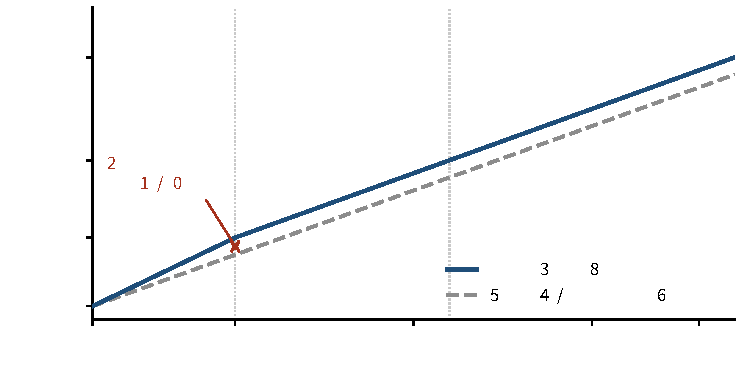
\includegraphics[width=0.78\textwidth]{fig-pwl.pdf}
\caption{变拍号下单一线性式与分段求和的偏差。虚线为原式（以段 2 的 BPI 相乘），
实线为真实的分段累计；两者自第 $5$ 小节分离，偏差恒为 $3840$ tick，
恰为一个 $4/4$ 小节。}
\label{fig:pwl}
\end{figure}

考虑一个三段变拍号工程，参数如表 \ref{tab:segdata}。

\begin{table}[htbp]
\centering
\caption{变拍号工程设定（$\mathrm{PPQ}=960$）}
\label{tab:segdata}
\begin{tabular}{@{}llcccc@{}}
\toprule
\thd{段} & \thd{小节范围} & \thd{拍号} & \thd{TPB} & \thd{每小节长度} \\
\midrule
段 1 & $1$--$4$   & $4/4$ & 960 & $4\times 960=3840$ \\
段 2 & $5$--$10$  & $3/4$ & 960 & $3\times 960=2880$ \\
段 3 & $11$--$18$ & $6/8$ & 480 & $6\times 480=2880$ \\
\bottomrule
\end{tabular}
\end{table}

求第 $5$ 小节第 $1$ 拍（\texttt{5.1.00}）的绝对 Tick。代入式 \eqref{eq:abs}
并使用段 2 的 $\mathrm{BPI}=3$：
\[
\bigl((5-1)\times 3 + (1-1)\bigr)\times 960 = 4\times 3\times 960 = 11520 \quad(\text{错}).
\]
而按分段累加，前 $4$ 个小节为 $4/4$，应有
\[
4\times 4\times 960 = 15360 \quad(\text{对}).
\]

\begin{观察}
误差为 $15360-11520 = 3840$ tick，\textbf{恰为一个 $4/4$ 小节}。
成因是：前 $4$ 个小节本是 $4/4$（每小节 $4$ 拍），却被原式用段 2 的
$\mathrm{BPI}=3$ 重算了一遍。
\end{观察}

误差「恰好等于一个小节」这一特征值得注意：它说明偏差并非舍入噪声，
而是结构性的——原式把一个分段线性映射误当成了直线。

\subsubsection{数学诊断}

式 \eqref{eq:abs} 把「小节序号 $\to$ tick」当作一次乘法即可求解的线性映射：
\begin{equation}
  \mathrm{Tick}(M) = k\cdot M + c \qquad(\text{一条直线}).
\end{equation}
但变拍号之后，该映射是\textbf{分段线性}的——每段斜率不同，其中第 $k$ 段的斜率为
\begin{equation}
  \label{eq:slope}
  \text{斜率}_k = \mathrm{BPI}_k \times \mathrm{TPB}_k .
\end{equation}

\begin{观察}[关键比喻]
原式以为坐标函数是一条直线，实际是一条折线。
对\textbf{直线}，一个乘法通吃；对\textbf{折线}，只能\textbf{分段求和}。
\end{观察}

\subsubsection{分段求和的通式}

设工程被划分为 $m$ 个拍号段，第 $s$ 段参数如表 \ref{tab:seg} 所示。

\begin{table}[htbp]
\centering
\caption{段表符号}
\label{tab:seg}
\begin{tabular}{@{}ll@{}}
\toprule
\thd{符号} & \thd{含义} \\
\midrule
$n_k$    & 第 $k$ 段所辖小节数 \\
$p_k$    & 第 $k$ 段每小节拍数（$=$ 拍号分子） \\
$d_k$    & 第 $k$ 段拍号分母 \\
$t_k$    & 第 $k$ 段每拍 tick 数 $=$ $\mathrm{PPQ}\times 4 / d_k$ \\
$\ell_k$ & 第 $k$ 段每小节 tick 数 $=$ $p_k \times t_k$ \\
\bottomrule
\end{tabular}
\end{table}

段起点 $S_s$ 为累计量：
\begin{equation}
  \label{eq:segstart}
  S_1 = 0,\qquad S_s = \sum_{k=1}^{s-1} n_k \,\ell_k .
\end{equation}
记 $A_s=\sum_{k<s} n_k$ 为前序各段的小节总数，则合并通式为
\begin{equation}
  \label{eq:master}
  \mathrm{AbsTick}(M,T) = \sum_{k<s} n_k \,\ell_k
  + \bigl((M-A_s-1)\,p_s + (T-1)\bigr)\,t_s .
\end{equation}

\begin{figure}[htbp]
\centering
\begin{示意图}
tick:   0                15360              32640
        |                  |                  |
        +---- 段1 ----+----- 段2 -----+---- 段3 ---->
        |  4 小节      |  6 小节       |  8 小节
        |  3840/小节   |  2880/小节    |  2880/小节
       S1=0          S2=15360        S3=32640
\end{示意图}
\caption{拍号段结构。斜率在第 $5$ 与第 $11$ 小节处改变，
故累积量必须分段求和。}
\label{fig:segments}
\end{figure}

\begin{注记}[「减一」的降级]
对比式 \eqref{eq:abs} 与式 \eqref{eq:master}：小节项由 $(M-1)$ 变为
$(M-A_s-1)$。\textbf{「减一」没有改变，但它从「全局减一」降级成了
「段内减一」。}
\end{注记}

\subsubsection{退化定理}

\begin{定理}[退化性]
当段数 $n=1$ 时，通式 \eqref{eq:master} 退化为原式 \eqref{eq:abs}。
\end{定理}

\begin{proof}
单段时 $A_1=0$ 且 $\sum_{k<1}(\cdot)=0$，代入 \eqref{eq:master} 得
$\mathrm{AbsTick}(M,T)=\bigl((M-1)\cdot\mathrm{BPI}+(T-1)\bigr)\cdot\mathrm{TPB}$，
与 \eqref{eq:abs} 逐项一致。
\end{proof}

该结论表明式 \eqref{eq:master} 是原式的\textbf{定义域扩充}而非替换：
原式定义域为段数 $n=1$，通式定义域为任意有限段数。在单拍号工程中替换实现
不改变任何既有行为，因而可以安全部署。

\begin{注记}[假设变成变量]
原式把「全曲同拍号」这一\textbf{假设}硬编码进了公式；通式把该假设本身
变成了一个\textbf{变量}（段表）。\textbf{假设变成变量，特例就长成了通式。}
\end{注记}

\subsubsection{推广后的验证}

对表 \ref{tab:segdata} 的工程，用式 \eqref{eq:master} 逐点计算并与宿主软件
实测对照，结果见表 \ref{tab:verify2}。

\begin{table}[htbp]
\centering
\caption{变拍号工程的实测对照}
\label{tab:verify2}
\begin{tabular}{@{}lcccc@{}}
\toprule
\thd{位置} & \thd{原式} & \thd{通式} & \thd{工具实测} & \thd{判定} \\
\midrule
\texttt{5.1.00}  & 11520 & \textbf{15360} & 15360 & 通式正确 \\
\texttt{9.2.00}  & ——    & \textbf{27840} & 27840 & 通式正确 \\
\texttt{11.1.00} & ——    & \textbf{32640} & 32640 & 通式正确 \\
\bottomrule
\end{tabular}
\end{table}

\texttt{9.2.00} 的手工核算如下：
\begin{align*}
  S_2 &= 15360,\\
  \text{段内} &= (M-A_2-1)\cdot p_2 + (T-1) = (9-4-1)\times 3 + (2-1) = 13,\\
  \Delta &= 13\times 960 = 12480,\\
  \text{合计} &= 15360 + 12480 = 27840 \;\checkmark .
\end{align*}

\subsubsection{取整误差}

式 \eqref{eq:tpb} 在分母为非 $2$ 的幂时须取整，误差可能随段数累积。
当 $d_k\in\{2,4,8,16,32\}$ 且 $\mathrm{PPQ}=960$ 时全部整除，无误差；
对罕见分母则须四舍五入。建议 $\mathrm{PPQ}$ 取高次幂
（$960 = 2^6\times 3\times 5$，可整除至 $/32$），以压缩该误差的出现概率。
本节仅给出观测，误差上界的严格证明留待后续工作（见第 \ref{sec:limit} 节）。

\subsection{精度分析}
\label{sec:precision}
绝对坐标的精度不由人的感知决定，而由系统的数值分辨率决定。
在 $\mathrm{PPQ}=960$ 下，一拍对应 $960$ tick，即
$1\ \mathrm{tick} \approx 1/960$ 拍。换算为物理时间，见表 \ref{tab:prec}。

\begin{table}[htbp]
\centering
\caption{不同分辨率下的时间精度（$120$ BPM）}
\label{tab:prec}
\begin{tabular}{@{}lcc@{}}
\toprule
\thd{PPQ} & \thd{1 tick 对应时间} & \thd{相对 $120$ BPM 一拍} \\
\midrule
$960$   & $\approx 0.5208$ ms & $1/960$ \\
$9600$  & $\approx 0.052$ ms  & $1/9600$ \\
$96000$ & $\approx 0.0052$ ms & $1/96000$ \\
\bottomrule
\end{tabular}
\end{table}

\begin{观察}
该精度在最高档位上已超出人类听觉的分辨极限，但其意义在于：
\textbf{这个精度不是由人的感知决定的，而是由计算机的计算精度决定的。}
坐标系本身没有能力上限，只有参数设定。
\end{观察}

为便于参照，可将该系统精度与人类演奏的时间控制能力对比。
顶尖演奏家的时间控制精度约在 $10\sim 20$ ms 量级；在 $120$ BPM 下一拍为
$500$ ms，故其精度约为 $1/50$ 拍。而 $\mathrm{PPQ}=960$ 对应
$1/960$ 拍 $\approx 0.5$ ms，已是该量级的约 $20$ 倍；
若取 $\mathrm{PPQ}=96000$，精度达 $0.005$ ms，完全超出任何人类的感知能力。

\begin{注记}
上述对比的意义不在于「机器比人准」，而在于说明：在本体系下，
误差来源是\textbf{参数设定}而非\textbf{能力上限}。
至于是否应当追求更高精度，是一个与审美和用途相关的问题。
一个音偏离标准网格 $0.0.12$，这既可以被读作「不够准」，
也可以被读作「这就是他的处理方式」——本体系只负责把它测出来。
\end{注记}

由此，传统表述中若干只能依靠感觉传递的修饰语，可以获得定量对应：

\begin{table}[htbp]
\centering
\caption{从定性修饰到定量偏移}
\label{tab:qualitative}
\begin{tabular}{@{}ll@{}}
\toprule
\thd{传统表述} & \thd{坐标化表述} \\
\midrule
「快一点」 & 提前 $3$ tick \\
「松一点」 & 延长 $2$ tick \\
「不够准」 & 偏移 $6$ tick \\
\bottomrule
\end{tabular}
\end{table}

\begin{注记}
表 \ref{tab:qualitative} 并不意味着审美判断可以被数值取代；
它只说明，当位置与长度被坐标化之后，\textbf{关于它们的描述}可以变得精确。
「精确」与「好听」是两个不同的问题，本体系只回答前者。
\end{注记}

\subsection{适用域与失效机理}
\label{sec:domain}
本节给出该形式的适用边界。这种自我限定在技术报告中并不常见，
但对工程部署是必要的——一个不知道自己何时失效的计算接口是危险的。

\subsubsection{拍号变化密度}

式 \eqref{eq:master} 的有效性随拍号变化密度而衰减。表 \ref{tab:domain} 给出
三类场景的对照。

\begin{table}[htbp]
\centering
\caption{按拍号变化密度划分的适用域}
\label{tab:domain}
\begin{tabular}{@{}llll@{}}
\toprule
\thd{场景} & \thd{原式} & \thd{通式} & \thd{正解} \\
\midrule
单一拍号 & 正确 & 正确（退化等价） & 任一 \\
少量变拍号 & 失效 & 正确 & 通式 \\
板式变化 / 散板 / 密集变拍 & 失效 & 失效 & 拍号事件表 + 二分查找 \\
\bottomrule
\end{tabular}
\end{table}

\subsubsection{参数复杂度}

\begin{figure}[htbp]
\centering
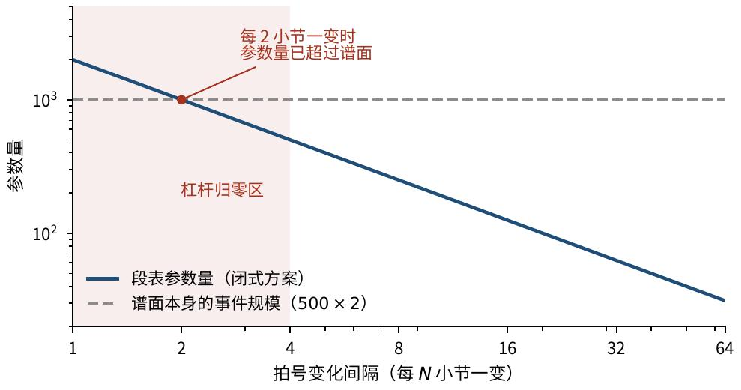
\includegraphics[width=0.78\textwidth]{fig-density.pdf}
\caption{参数量随拍号变化密度的增长（$500$ 小节工程，平均每小节 $2$ 个事件）。
横轴为「每 $N$ 小节一变」，纵轴取对数。段表参数量按连续值绘制——
实际段数须取整，取整会使曲线成为阶梯，此处略去以看清趋势。
密度升高时参数量随之增长，并在每 $2$ 小节一变处超过谱面本身的事件规模，
闭式相对于直接罗列数据的杠杆随之归零。}
\label{fig:density}
\end{figure}

\begin{table}[htbp]
\centering
\caption{参数规模随拍号变化密度的增长}
\label{tab:params}
\begin{tabular}{@{}ll@{}}
\toprule
\thd{场景} & \thd{参数量} \\
\midrule
单一拍号 & $\approx 3$ \\
$3$ 段变拍 & $3\times 4 = 12$ \\
密集变拍（每 $2$ 小节一换，$500$ 小节） & $\approx 1000$ \\
\bottomrule
\end{tabular}
\end{table}

参数量随拍号变化密度\textbf{线性增长}，其曲线见图 \ref{fig:density}；
表 \ref{tab:params} 给出三个代表性取值。

\begin{观察}[失效机理]
当拍号变化密度趋近「每小节一变」时，参数规模趋近谱面本身，
公式相对于直接罗列数据的杠杆归零。
\end{观察}

此时的正解并非「更优的公式」，而是\textbf{范式切换}：存储拍号事件表，
查询改用 $O(\log n)$ 二分查找。主流 DAW 的工程实现正是如此，
且均不对外提供变拍号情形的闭式公式 \footnote{同前注。}。

\begin{注记}[本式的定位]
式 \eqref{eq:master} 是「低密度变拍号」场景下的一个 $O(1)$ 计算接口。
它不是数学发现，也不是通用解法，而是一个边界明确的小工具；
其价值上限由拍号变化密度决定。
\end{注记}

\subsubsection{反向映射的不可替代性}

式 \eqref{eq:abs} 与式 \eqref{eq:master} 的价值在正反两个方向上并不对称：

\begin{table}[htbp]
\centering
\caption{正反两个方向的可替代性}
\label{tab:asym}
\begin{tabular}{@{}lll@{}}
\toprule
\thd{方向} & \thd{形式} & \thd{可否人工替代} \\
\midrule
正向 & $\mathrm{Position} \to \mathrm{AbsTick}$ & 可以，手算亦可 \\
反向 & $\mathrm{AbsTick} \to \mathrm{Position}$ & \textbf{不可以}，须依赖累计边界 $S_s$ \\
\bottomrule
\end{tabular}
\end{table}

原因在于，位置与 tick 之间是分片线性、严格单调的双射，反向求解的落脚点正是
各段累计边界 $S_s$；脱离了这串边界，反向映射无唯一解可循。

\subsubsection{三条硬前提}
\label{sec:limit}

该形式的成立依赖以下前提，超出即不适用。

\begin{enumerate}[leftmargin=2.2em,itemsep=0.15em,topsep=0.2em]
  \item \textbf{前提 A：段表已知。} 式 \eqref{eq:master} 不负责求解段表。
        由命题 1，拍号图无法由 tick 序列反推（不适定），故段表必须由外部提供
        （工程数据或乐谱标注）。
  \item \textbf{前提 B：段表如实反映工程的拍号图。} 本式不负责校验。
  \item \textbf{前提 C：「一拍」的定义与宿主软件的约定一致。} 在 $6/8$ 下，
        宿主软件可能将一拍定义为八分音符（$\mathrm{TPB}=480$），
        而乐理上 $6/8$ 通常读作两个附点四分音符。换用不同约定，读数随之改变。
\end{enumerate}

\begin{注记}
本式是计算器，不是审计员：它不做前提校验。
准确的表述是——\textbf{在拍单位约定一致、且段表正确的前提下，通式精确成立。}
\end{注记}

% ---------------------------------------------------------------------------
%  推论一：事件层
% ---------------------------------------------------------------------------
\section{推论一：事件的坐标化}
\label{sec:event}

本节说明第一项推论：一旦位置成为绝对坐标，「什么是一个音乐事件」这个问题
便不再是音乐学判断，而退化为坐标上的一个纯算术条件——\textbf{纵向值是否
发生改变}。休止也因此不再需要特殊处理。
\subsection{事件视角与空事件}

记谱传统以「音高的有无」为基本判据：有声为音符，无声为休止。这一划分在定位
问题上引入了不必要的特殊处理——休止成了「空白」，需要额外规则描述。

本文采用另一种视角：把音乐视为由若干离散\textbf{事件}构成的时间序列，
每个事件具有独立的起止时刻与音高属性。

\begin{定义}[空事件]
\textbf{空事件}（Empty Event）指音高属性为空、但具有明确起止时刻的事件。
休止即一种空事件。
\end{定义}

\begin{观察}
不以「音高的有无」为基本判据，而以「事件的起止」为统一的时间定位依据，
则所有音乐元素（含休止）在坐标系中均具有确定位置。
\end{观察}

由于所有事件均以起止时刻定义，相邻事件的终点与起点首尾相接，
在连续时间轴表示下构成一条不间断的\textbf{事件链}。任意相邻事件的衔接点
构成该时刻的唯一事件边界。

\begin{观察}
在事件视角下，音乐时间轴上不存在「空白」——每一时刻均归属于某一事件，
不存在任何歧义或未定义区域。
\end{观察}

\subsection{事件的判据}

\begin{figure}[htbp]
\centering
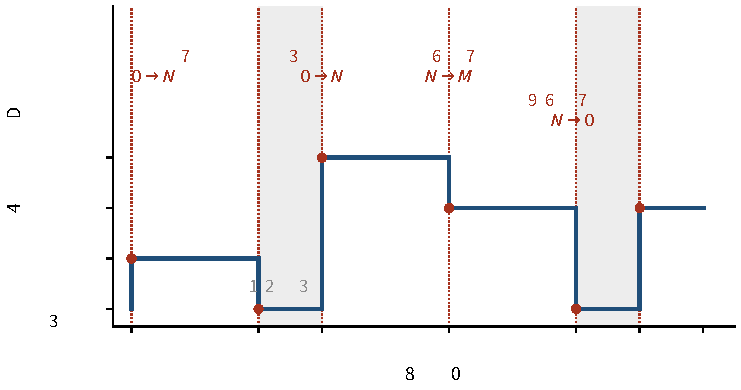
\includegraphics[width=0.78\textwidth]{fig-event.pdf}
\caption{事件判据的几何含义。纵轴为等距排列的纵向值行（标签为真实 MIDI 音高），
横轴为绝对 tick。阶梯的每一次跳变即一个事件；四类边界
（音符起始、连奏起始、断奏起始、休止结束）由同一条件触发。
灰色区间为「空事件」，即休止。}
\label{fig:eventcriterion}
\end{figure}

将连续时间按绝对 tick 离散化后，每个时间切片上存在唯一的纵向状态。
据此给出事件判据：

\begin{定义}[事件]
\textbf{事件 $=$ 纵向值发生改变的瞬间。} 其中纵向值取绝对 MIDI 音高，
取 $0$ 表示休止。
\end{定义}

该判据使四类在记谱上彼此不同的现象退化为同一检测逻辑，如表 \ref{tab:events}
所示。

\begin{table}[htbp]
\centering
\caption{四类事件在同一判据下的表述}
\label{tab:events}
\begin{tabular}{@{}lll@{}}
\toprule
\thd{事件类型} & \thd{纵向值变化} & \thd{附加条件} \\
\midrule
音符起始 & $0 \to N$ & —— \\
连奏起始 & $N \to M$ & 时刻 $T$ 时 $N$ 尚未结束（存在交叠） \\
断奏 / 休止起始 & $N \to 0$ & —— \\
休止结束 & $0 \to N$ & 与音符起始同属一类 \\
\bottomrule
\end{tabular}
\end{table}

\subsection{事件链递推}

由事件链的衔接性质可得递推关系：
\begin{align}
  E_1^{\,start} &= \mathrm{AbsTick}(M_1,T_1), \label{eq:c1}\\
  E_i^{\,end}   &= E_i^{\,start} + \delta_i, \label{eq:c2}\\
  E_{i+1}^{\,start} &= E_i^{\,end}, \label{eq:c3}
\end{align}
其中 $\delta_i$ 为第 $i$ 个事件的时值。式 \eqref{eq:c3} 即「前事件结束等于
后事件起始」，它并非音乐理论命题，而是时间轴连续性在离散坐标下的直接推论。

\textbf{单点定位}是已知某一音符的位置；\textbf{全局定位}是从起始音出发，
借助式 \eqref{eq:c3} 一次递推生成全部事件。二者的差别仅在于是否施加该递推。

\subsection{全量扫描算法}

上述逻辑在实现上等价于一次自时间轴起点至终点的全量扫描：

\begin{museCode}[language=Python]
def scan_events(states):
    """states[t] = 第 t 个绝对 tick 上的纵向值 (0 表示休止)"""
    events = []
    for t in range(1, len(states)):
        if states[t] != states[t - 1]:          # 纵向值发生改变
            events.append((t, states[t - 1], states[t]))
    return events

def classify(prev, cur):
    if prev == 0 and cur != 0: return "onset"
    if prev != 0 and cur == 0: return "rest"
    if prev != 0 and cur != 0: return "legato"
\end{museCode}

\vspace{-0.3em}
\begin{figure}[htbp]
\centering
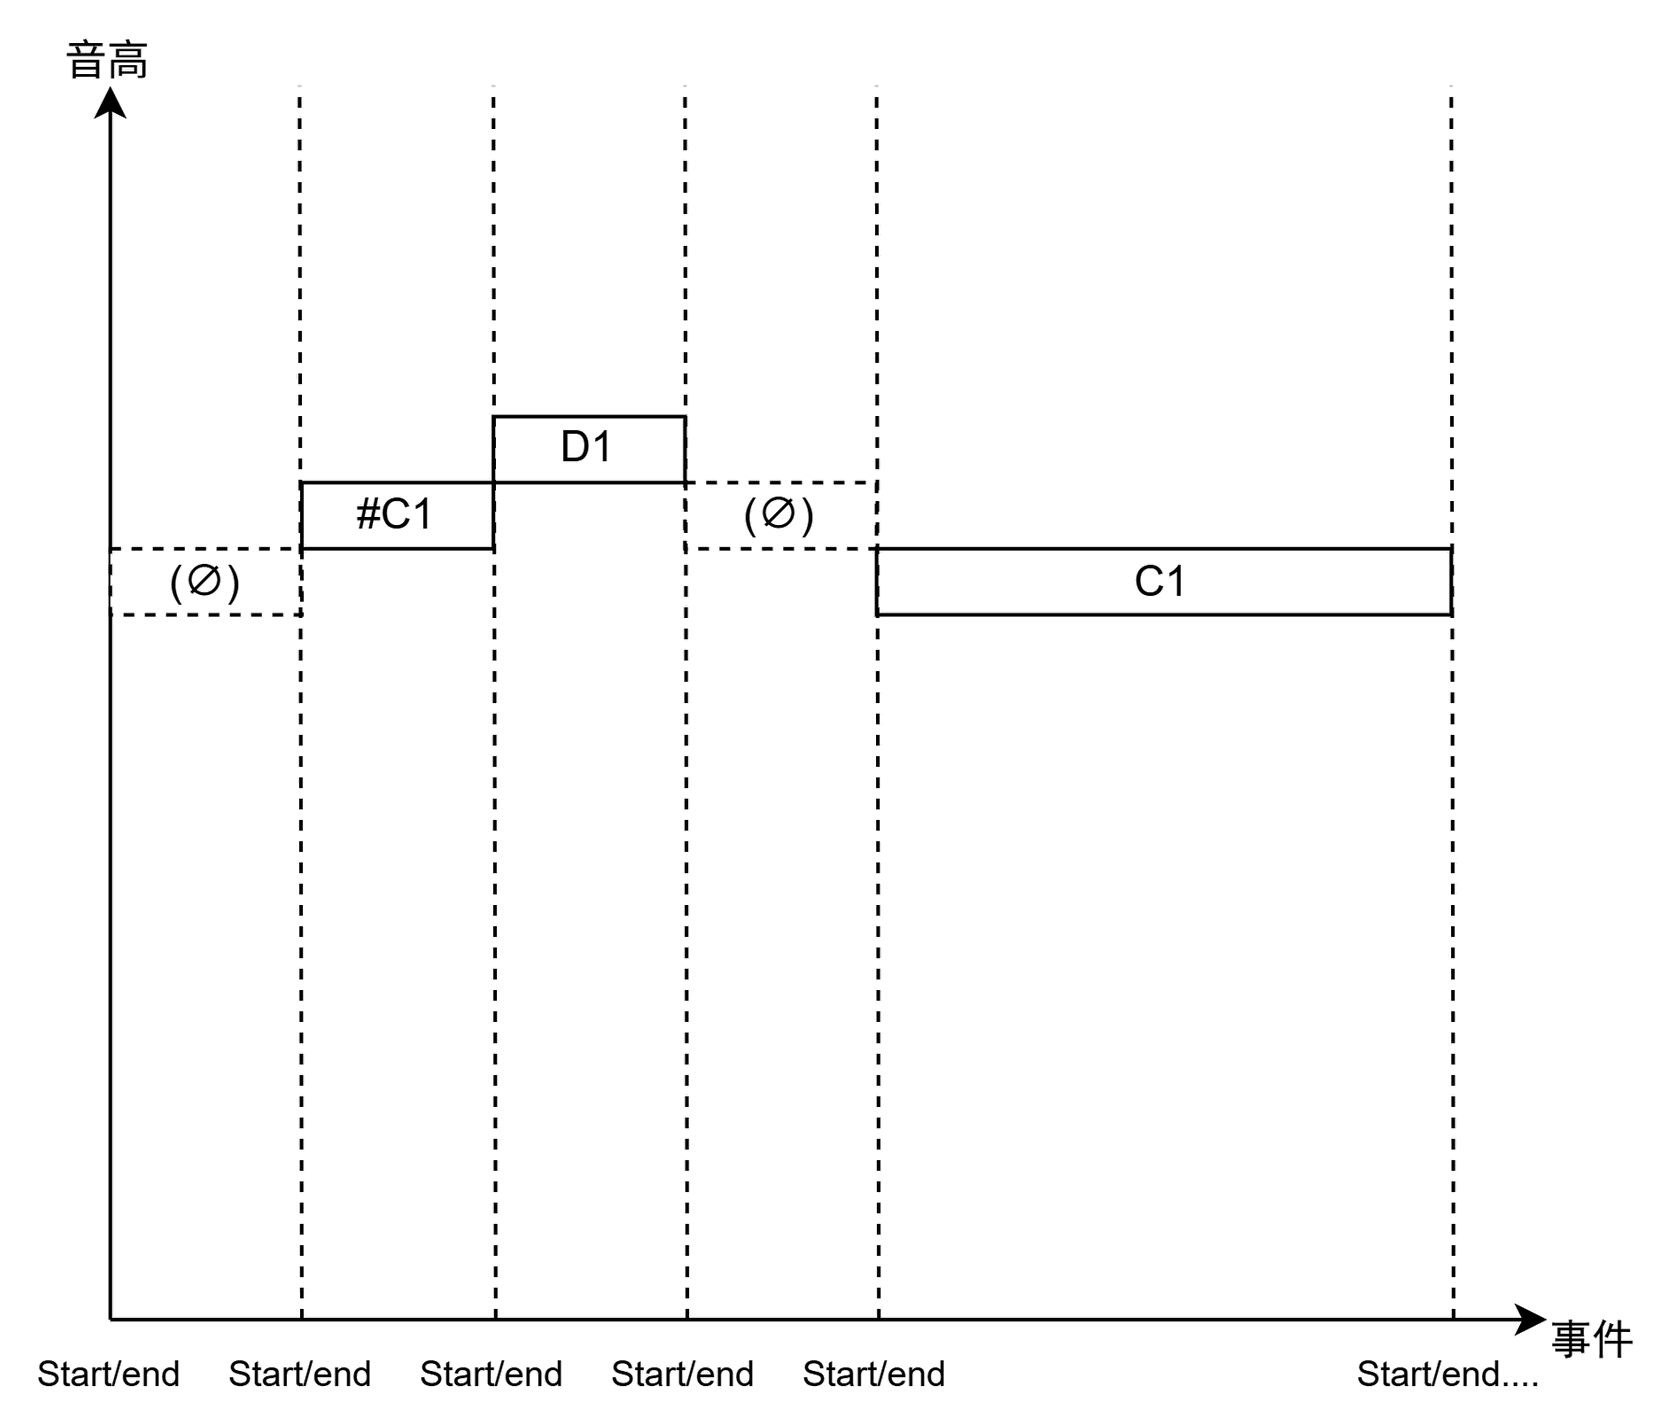
\includegraphics[width=0.64\textwidth]{fig2-event-draw.png}
\caption{事件绘制。实线块为音符事件，虚线块为空事件（休止），
二者共享同一套起止结构。}
\label{fig:event}
\end{figure}

\begin{figure}[htbp]
\centering
\begin{minipage}[t]{0.485\textwidth}
  \centering
  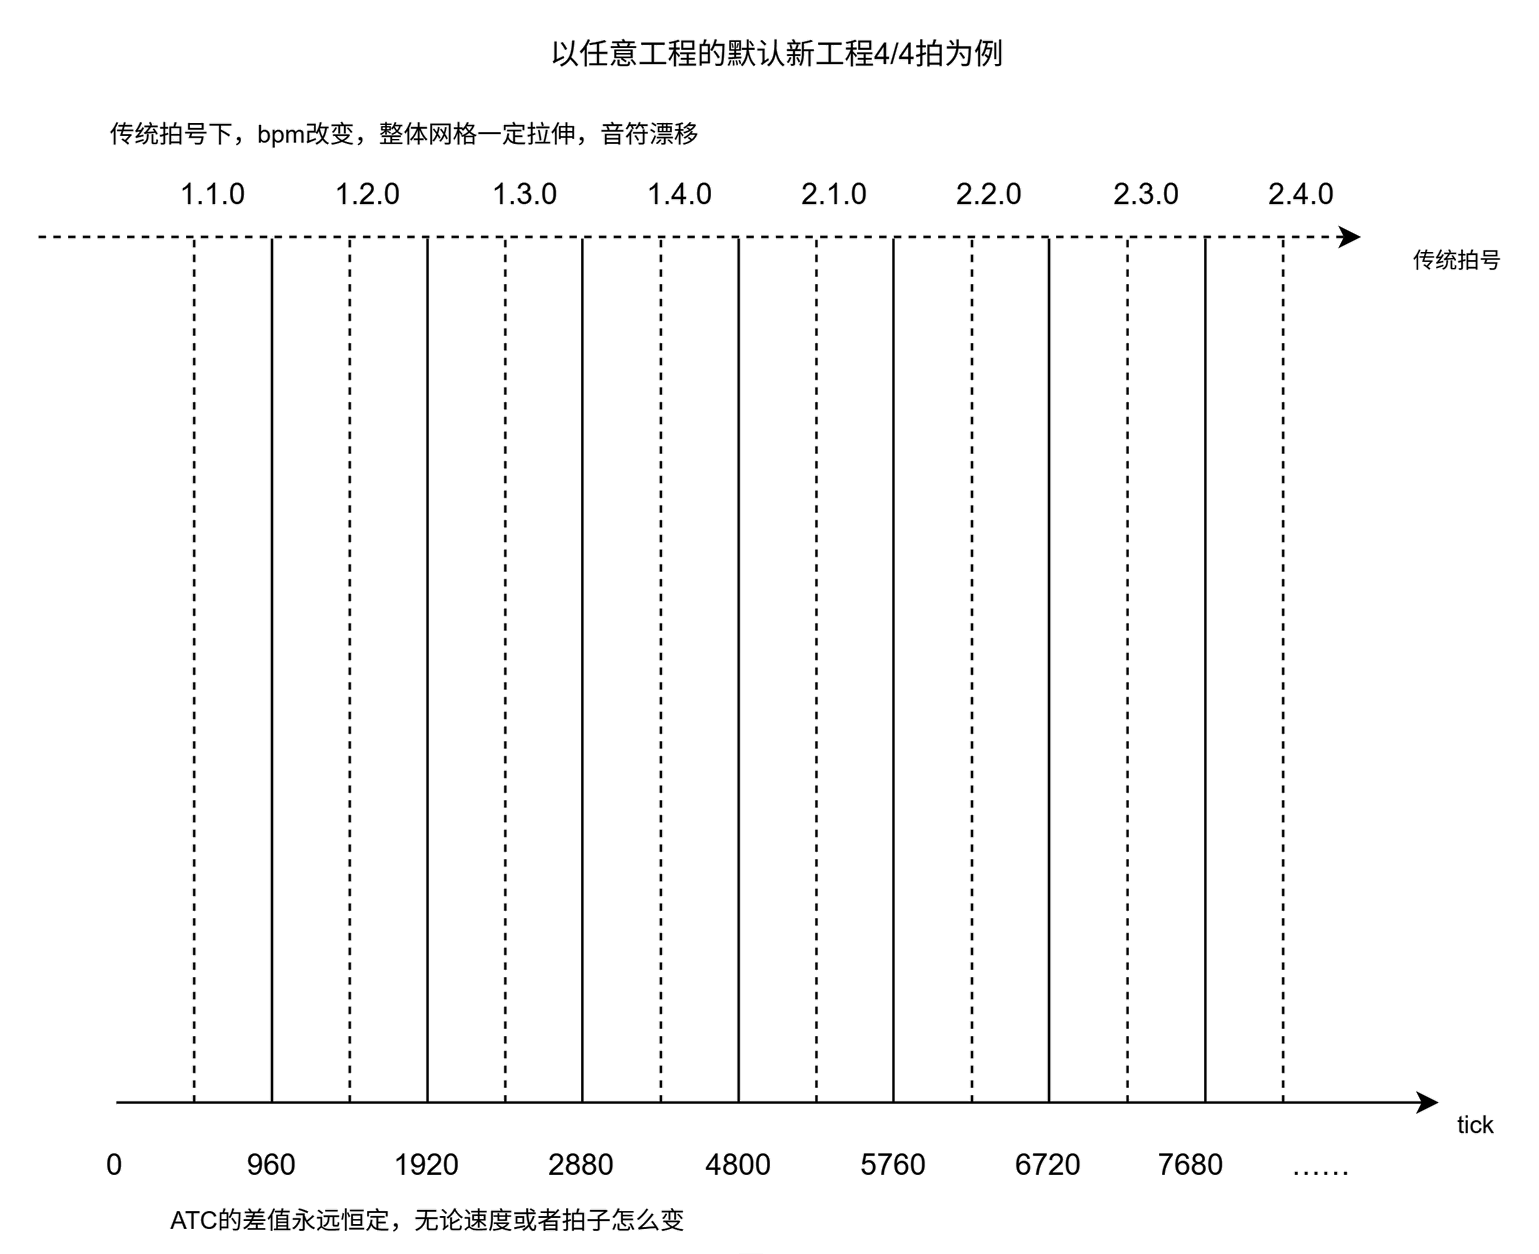
\includegraphics[width=\linewidth]{fig1-tick-coord.png}\\[1pt]
  {\sffamily\small (a) 绝对 Tick 刻度}
\end{minipage}\hfill
\begin{minipage}[t]{0.485\textwidth}
  \centering
  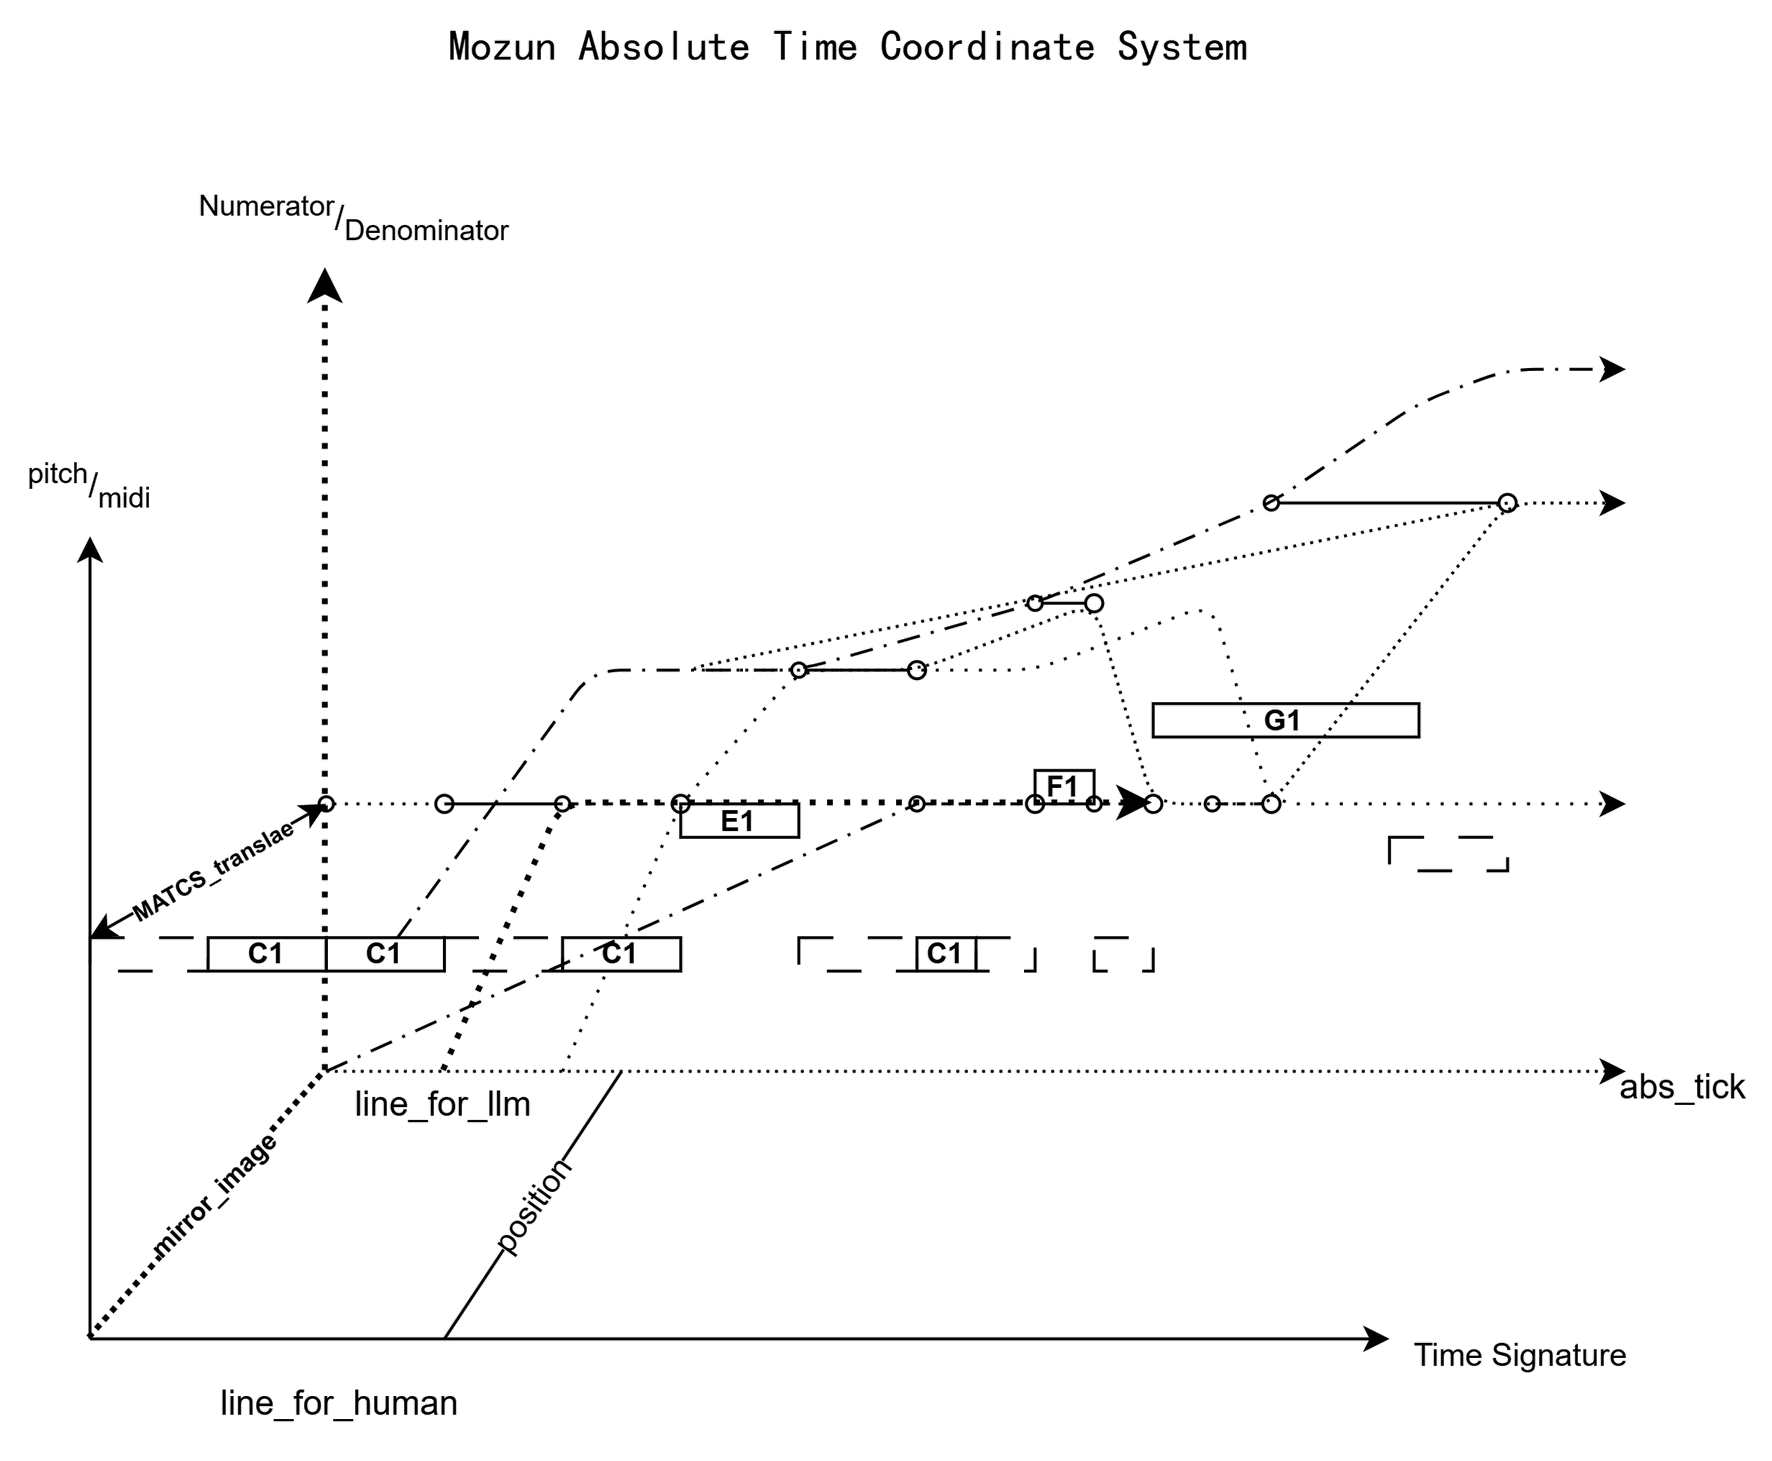
\includegraphics[width=\linewidth]{fig3-matcs.png}\\[1pt]
  {\sffamily\small (b) 纵向映射与读取}
\end{minipage}
\caption{音乐事件的时空坐标化。横轴提供唯一刻度，纵轴提供事件判据。}
\label{fig:radar}
\end{figure}

\section{推论二：技法与声部的坐标化}

本节说明第二项推论：连奏、断奏、大跳与声部归属，都不需要另行定义——
它们是坐标差的直接读数。把它们写成独立方法是一种误导；
准确的说法是，\textbf{它们都是核心坐标系的导出量}。

\subsection{事件关系的量化}
\label{sec:relation}
\subsubsection{统一判据}

有了绝对坐标，「连奏」与「断奏」这类定性描述可以获得统一的定量形式。
设相邻事件 $A$、$B$，定义差值
\begin{equation}
  \label{eq:gap}
  \Delta = A^{\,end}_{\mathrm{tick}} - B^{\,start}_{\mathrm{tick}} .
\end{equation}
则
\begin{equation}
  \label{eq:relation}
  \Delta > 0 \;\Rightarrow\; \text{连奏（交叠)},\qquad
  \Delta = 0 \;\Rightarrow\; \text{完美连接},\qquad
  \Delta < 0 \;\Rightarrow\; \text{断奏（间隙)}.
\end{equation}

按 $|\Delta|$ 的大小可进一步分级，如表 \ref{tab:articulation} 所示。

\begin{table}[htbp]
\centering
\caption{连奏与断奏的程度分级（$\mathrm{PPQ}=960$）}
\label{tab:articulation}
\begin{tabular}{@{}lcc@{}}
\toprule
\thd{程度} & \thd{$|\Delta|$ 范围} & \thd{说明} \\
\midrule
轻微 & $0 \sim 120$ tick & 约八分之一拍以内 \\
明显 & $120 \sim 480$ tick & 半拍以内 \\
强烈 & $> 480$ tick & 超过半拍，连奏时构成延留音 \\
\bottomrule
\end{tabular}
\end{table}

\subsubsection{大跳}

设相邻事件音高为 $Y_1$、$Y_2$，则大跳判据为
\begin{equation}
  \label{eq:leap}
  |Y_2 - Y_1| \geq 5 \;\Rightarrow\; \text{大跳}.
\end{equation}
阈值 $5$ 对应纯四度，即三度以内（$\leq 4$ 半音）不计为大跳。
表 \ref{tab:interval} 给出常见音程的判定。

\begin{table}[htbp]
\centering
\caption{音程与大跳判定}
\label{tab:interval}
\begin{tabular}{@{}lcc@{}}
\toprule
\thd{音程} & \thd{半音数} & \thd{判定} \\
\midrule
三度以内 & $\leq 4$ & 非大跳 \\
纯四度 & $5$ & 大跳 \\
增四度 / 减五度 & $6$ & 大跳 \\
纯五度 & $7$ & 大跳 \\
小六度 & $8$ & 大跳 \\
八度及以上 & $\geq 12$ & 大跳 \\
\bottomrule
\end{tabular}
\end{table}

\subsubsection{二维联动}

式 \eqref{eq:relation} 与式 \eqref{eq:leap} 分别刻划横向与纵向，
二者联合可将相邻事件归入四类，见表 \ref{tab:2d}。

\begin{table}[htbp]
\centering
\caption{横向差值与纵向音高差的联合分类}
\label{tab:2d}
\begin{tabular}{@{}lll@{}}
\toprule
\thd{横向（$\Delta$）} & \thd{纵向（$|Y_2-Y_1|$）} & \thd{判定} \\
\midrule
交叠 $>0$ & $\geq 5$ & 连奏大跳 \\
交叠 $>0$ & $<5$    & 连奏级进 \\
间隙 $>0$ & $\geq 5$ & 断奏大跳 \\
间隙 $>0$ & $<5$    & 断奏级进 \\
\bottomrule
\end{tabular}
\end{table}

\begin{注记}
这一分类的意义在于：它把「这段旋律起伏如何」这类整体印象，
分解为可以逐对事件统计的局部量。第 \ref{sec:case} 节的案例即利用这一分解
比较两份旋律的差异。
\end{注记}

\subsection{声部分离与旋律线追踪}
\label{sec:voice}
\subsubsection{问题的界定}

声部分离是旋律追踪、和声分析与结构化编辑的共同前置任务。传统做法依赖音区
先验（例如「右手高于左手」），但这一先验在声部交叉处失效。

\begin{定义}[声部区分的相对性]
声部区分不是绝对的（例如「钢琴右手一定高于 C4」），而是相对的——
取决于当前这段音符的具体音高范围。
\end{定义}

这一定义意味着声部分离应当是一个\textbf{自适应的无监督划分}问题，
而不是一个固定阈值的分类问题。本文给出三层递进的判据：音区粗分（\ref{subsec:yaxis}）、
递归细分（\ref{subsec:recursive}）与时间连续性（\ref{subsec:line}）。

\subsubsection{音区粗分}
\label{subsec:yaxis}

在纵向轴上，四声部合唱（SATB）通常具有明确的音区分层。设纵向坐标经八度归一
后为 $Y'$，则只需划定一个简单阈值即可完成粗分：$Y'$ 高于阈值的归入高声部，
低于阈值的归入低声部。

以一段钢琴谱为例，右手旋律位于中高音区，左手伴奏位于中低音区。若以
$Y'=-0.5$ 为阈值，右手音符（$Y'\in\{0,+1\}$）与左手音符（$Y'\in\{-1,-2\}$）
即可被分拣到两个声部列表。

\begin{注记}
该粗分的本质是把一个二维点阵在 $Y'$ 轴上做「等高线」切分。
它在四部和声出现八度交叉时会失效，故须由后续判据补足。
\end{注记}

\subsubsection{递归细分}
\label{subsec:recursive}

为摆脱固定阈值，可取递归二分策略：先定位全局最高音与最低音，取其中点将音高
空间分为上下两半；再对每一半分别取中点，最终得到三个区间。
该过程等价于一种自适应的无监督聚类。

\begin{table}[htbp]
\centering
\caption{三层递进的声部判据}
\label{tab:voice3}
\begin{tabular}{@{}llll@{}}
\toprule
\thd{层次} & \thd{依据} & \thd{适用} & \thd{失效条件} \\
\midrule
音区粗分 & $Y'$ 轴阈值 & 音区分离明显 & 声部八度交叉 \\
递归细分 & 音高分布密度低谷 & 无先验音区 & 两音区重叠严重 \\
时间连续性 & 音尾—音头最近距离 & 声部交叉 & 需先解决休止缺口 \\
\bottomrule
\end{tabular}
\end{table}

\subsubsection{连线法}
\label{subsec:line}

\begin{定义}[连线法]
在任意音的音尾处，该音的音尾自动与当前\textbf{距离最接近}的音符的音头匹配为
一个声部，进行连线。若交叠则无需考虑，必然为同一 声部；若一个音同时与前一个音
的上下声部出现同样的距离，则反推此逻辑，此声部必定为中声部。
\end{定义}

判据分为两条逻辑。

\textbf{逻辑一：音尾与最近音头匹配。} 对音符 $A$，扫描其后的全部音符起始位置，
取距离最近者为后继：若存在交叠（$A$ 的音尾晚于后继的音头），必然同声部；
若无交叠但距离最近，亦归为同声部。

\begin{注记}
在复调音乐中，同一声部的音符通常首尾相接或略微交叠，很少出现巨大的时间间隙。
用「最近距离」判断，比「是否在同一音区」准确得多——因为声部交叉时，
高音声部可能暂时低于中音声部，但\textbf{时间上的连续性不会断开}。
\end{注记}

\textbf{逻辑二：等距排除法。} 设音符 $C$ 的起始位置与上方音符 $A$ 的音尾距离，
等于与下方音符 $B$ 的音尾距离，则 $C$ 不属于上声部也不属于下声部，
必定为中声部。

\begin{观察}
「等距排除法」解决的是声部归属的模糊地带：当一个音正好卡在上下两个声部之间时，
不靠音高判断，而靠距离的等值关系反推。其数学含义是：若 $C$ 与 $A$、$B$ 等距，
则 $C$ 在时间轴上独立于 $A$、$B$ 的连线关系，必然属于第三个独立声部。
\end{观察}

两条逻辑协同的流程为：自第一个音起遍历；每个音的音尾寻找距离最近的音头；
交叠则直接锁定同声部；等距则反推为中声部；连成线后输出旋律线。

\subsubsection{虚拟桥：休止缺口的桥接}

\begin{figure}[htbp]
\centering
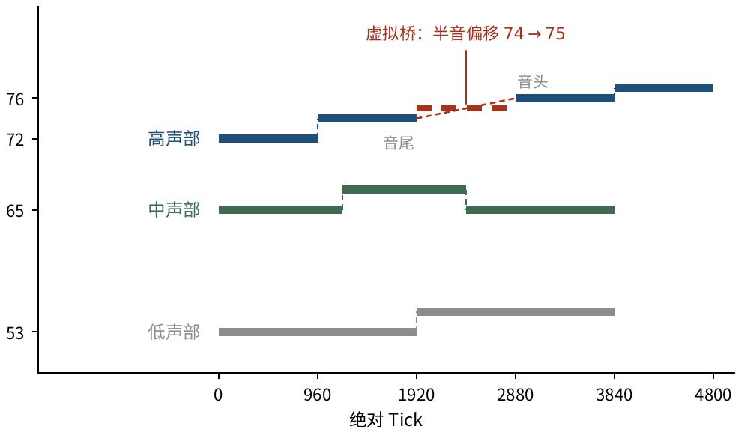
\includegraphics[width=0.78\textwidth]{fig-voice.pdf}
\caption{声部分离与虚拟桥。三个声部以横条表示，虚线为「音尾至最近音头」的连线。
高声部在第 $1920$–$2880$ tick 之间存在休止缺口，连线因此中断；
以音高偏移半音的虚拟音符搭桥后（红色虚条），连线得以贯通；
追踪结束后桥被拆除，其占用的区间即记为休止。}
\label{fig:voicebridge}
\end{figure}
\label{subsec:bridge}

连线法依赖时间连续性，而休止会在事件链上留下缺口，使追踪中断。
本文的处理方式是引入\textbf{虚拟桥}。

\begin{定义}[虚拟桥]
在休止处假设一个虚拟音符，自当前音尾开始，以\textbf{半音偏移}取值并持续延伸，
直到遇到下一个真实音符时消失，从而让连线法可以自然地完成
「真实音 $\to$ 虚拟音 $\to$ 真实音」的连接。
\end{定义}

之所以采用半音偏移而非同音高，是因为同一音高不可能交叠
（受 MIDI 协议与物理演奏限制）。若虚拟音与真实音同音高，连线法会遇到逻辑冲突；
半音偏移（如 $\mathrm{C2}\to\#\mathrm{C2}$）既避免了同音高，
又保持了最小音程差异，因而不影响声部归属判断。

\begin{观察}[过河拆桥]
虚拟音符的唯一任务是用其长度「填满」那段沉默，从而把算法上的缺口连接上。
一旦追踪完成，算法即判定「这是虚拟音符，不输出到最终结果」。
但\textbf{它原本占据的精确时间长度会被原封不动地保留下来}——
该长度正是从一个音结束到下一个音开始之间的自然沉默时间。
\end{观察}

因此，休止不需要任何额外的特殊处理：它是被桥接、被追踪、再被拆除的，
而拆除后留下的那段长度即构成休止事件。这与第 \ref{sec:event} 节把休止定义为
空事件的立场一致——休止不是「无」，而是一段有起止的时间。

% ---------------------------------------------------------------------------
%  推论三：结构层
% ---------------------------------------------------------------------------
\section{推论三：结构的坐标化}
\label{sec:gen}

本节说明第三项推论：作品的段落结构可以表示为同一坐标轴上的区间递推划分，
动机发展则表示为该坐标平面上的几何变换。两者都是坐标运算，
不需要对音乐作任何「理解」。
绝对坐标解决的是「事件在哪里」。一个自然的问题是：同一套坐标能否反过来
用于生成，即「事件应当在哪里」。本节给出一个三层架构，
其设计原则是把\textbf{能被生成的东西}与\textbf{不被允许的东西}分离处理。

\subsection{三条公理}

\begin{enumerate}[leftmargin=2.2em,itemsep=0.15em,topsep=0.2em]
  \item \textbf{时间总守恒。} 设作品总时长为 $T_{\mathrm{total}}$（以 tick 计），
        被划分为 $n$ 个段落，第 $i$ 段时长为 $S_i$，则
        \begin{equation}
          \label{eq:conservation}
          T_{\mathrm{total}} = \sum_{i=1}^{n} S_i .
        \end{equation}
  \item \textbf{递归划分。} 任一段落可继续划分：$S_i = \sum_j s_{ij}$。
  \item \textbf{结构模板。} 作品的段落组织是一个序列模式：
        $\mathrm{Structure} = \mathrm{pattern}(S_1,\dots,S_n)$。
\end{enumerate}

\begin{注记}
公理 \eqref{eq:conservation} 与第 \ref{sec:coord} 节的坐标定义是同一件事的
两种说法：前者约束总长度，后者给出每个事件的位置。二者结合，
使「任意划分总时间」成为一个可计算操作。
\end{注记}

\subsection{结构层：时间守恒下的递归划分}

结构的合法性由式 \eqref{eq:conservation} 保证。以常见曲式为例，
约束的具体形式见表 \ref{tab:form}。

\begin{table}[htbp]
\centering
\caption{常见曲式的时间守恒约束}
\label{tab:form}
\begin{tabular}{@{}ll@{}}
\toprule
\thd{曲式} & \thd{约束} \\
\midrule
$A$--$B$--$A$ & $T = S_A + S_B + S_A$ \\
$A$--$B$--$C$--$A$ & $T = S_A + S_B + S_C + S_A$ \\
$A$--$B$--$A$--$B$--$A$ & $T = S_A + S_B + S_A + S_B + S_A$ \\
\bottomrule
\end{tabular}
\end{table}

该约束同时容纳方整与非方整结构：$S_A=S_B=S_A=16$ 与
$S_A=13,\;S_B=17,\;S_A=18$ 给出相同的 $T=48$。
换言之，守恒只约束总和，不约束分配；分配是否合理是审美问题而非数学问题。

\begin{定理}[曲式递归]
任何曲式结构都可以递归地细分为更小的曲式结构，且该递归可无限进行。
\end{定理}

\begin{proof}
对分层数 $k$ 作归纳。基础情形 $k=1$：单个段落自身满足
$S_A=\sum_j s_{aj}$，即一段可划分为若干子段。归纳步：设第 $k$ 层成立，
即 $p_i=\sum_j p_{ij}$；则对每个 $p_{ij}$ 重复同样论证即可得到第 $k+1$ 层。
由此可从乐章划分递归至乐段、乐句、动机，直至单个音符。
\end{proof}

该定理意味着一部交响曲的 $A$--$B$--$A$ 结构与一段 $16$ 小节旋律的
$a$--$b$--$a'$ 结构在数学上同构。

\subsection{生成层：动机的几何变换}

\begin{定义}[动机]
动机是带坐标的有序音符序列 $M=\{n_1,\dots,n_k\}$，
其中每个音符 $n_i=(x_i,y_i)$，$x_i$ 为起始绝对 tick，
$y_i$ 为 MIDI 音高编号。
\end{定义}

在式 \eqref{eq:event} 的二维坐标下，全部传统动机发展技法可被写成统一的
几何变换，见表 \ref{tab:motive}。

\begin{table}[htbp]
\centering
\caption{动机发展技法的几何变换形式}
\label{tab:motive}
\begin{tabular}{@{}lll@{}}
\toprule
\thd{技法} & \thd{变换} & \thd{作用维度} \\
\midrule
重复 & $n_i' = (x_i + \Delta x,\; y_i)$ & 时间平移 \\
倒影 & $n_i' = (x_i,\; 2Y_{\mathrm{ref}} - y_i)$ & 关于轴 $Y_{\mathrm{ref}}$ 的纵向反射 \\
逆行 & $M' = \{n_k, n_{k-1}, \dots, n_1\}$ & 序列反转 \\
扩大 & $n_i' = (x_i \cdot \lambda,\; y_i),\;\lambda>1$ & 时间缩放 \\
缩小 & $n_i' = (x_i \cdot \lambda,\; y_i),\;0<\lambda<1$ & 时间缩放 \\
\bottomrule
\end{tabular}
\end{table}

变换可以复合，例如
$M' = \mathrm{scale}_x\bigl(\mathrm{reflect}(M, Y_{\mathrm{ref}}),\,2.0\bigr)$
表示先倒影再扩大两倍。

\begin{观察}
在坐标表示下，动机发展不需要「理解音乐」，只需执行代数运算。
这与其他推理任务并无本质差别。
\end{观察}

\subsection{过滤层：约束的可计算化}

生成层只负责「可以这样排」，不负责「不允许那样排」。后者由过滤层承担。

\begin{定理}[过滤函数的存在性]
给定任意音乐约束 $C$，存在一个可计算的过滤函数 $F_C$，
使得 $F_C(\text{sequence})$ 返回真当且仅当该序列满足 $C$。
\end{定理}

\begin{proof}[证明思路]
约束 $C$ 只需可被判定，即可写为对序列的谓词；逐个检验序列元素即可得到
$F_C$。该构造不保证效率，但保证存在性。
\end{proof}

表 \ref{tab:filter} 列出若干常用约束及其过滤函数形式。

\begin{table}[htbp]
\centering
\caption{常用约束与对应过滤函数}
\label{tab:filter}
\begin{tabular}{@{}llp{5.0cm}@{}}
\toprule
\thd{约束} & \thd{过滤函数} & \thd{效果} \\
\midrule
调性 & $p \bmod 12 \in C_{\mathrm{major}}$ & 保证音符落在指定音阶内 \\
音域 & $y_{\min} \le y \le y_{\max}$ & 确保不超出乐器音域 \\
连奏 & $\lnot(\Delta>0 \land y_i = y_{i+1})$ & 排除同音高交叠 \\
和声 & $p \in$ 和弦模板 & 约束纵向同时性 \\
比例 & $S_i/S_j \in [r_{\min}, r_{\max}]$ & 约束段落比例 \\
\bottomrule
\end{tabular}
\end{table}

\begin{注记}
「同音高不可能交叠」这一过滤条件与第 \ref{subsec:bridge} 节虚拟桥采用
半音偏移的理由是同一个：它既是物理约束，也是算法一致性约束。
\end{注记}

多个约束以合取方式叠加：
\begin{equation}
  \label{eq:filterchain}
  F_{\mathrm{total}} = F_1 \land F_2 \land \cdots \land F_k .
\end{equation}
任何通过式 \eqref{eq:filterchain} 全部过滤器的序列，按构造即满足全部约束。
新增需求只需追加一个过滤函数，无需改动生成层。

\subsection{闭环与总体形式}

\begin{figure}[htbp]
\centering
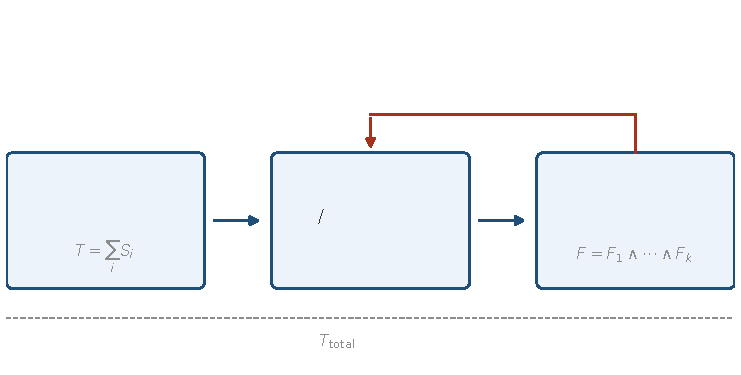
\includegraphics[width=0.78\textwidth]{fig-arch.pdf}
\caption{结构—生成—过滤三层闭环。结构层以时间守恒约束段落划分，
生成层以几何变换产生动机变体，过滤层判定结果是否满足音乐约束；
被拒绝的结果回退到生成层重新变换，而总时长约束在全过程中保持不变。}
\label{fig:arch}
\end{figure}

三层的关系为：结构层决定「多长、分几段」，生成层决定「音符怎么排」，
过滤层决定「哪些音不能用」。三者构成闭环——生成结果若被过滤层拒绝，
即回退到生成层重新变换，而总时长约束始终保持不变。据此，音乐生成可写为
\begin{equation}
  \label{eq:generate}
  \text{生成} = \underbrace{\text{时间守恒下的递归划分}}_{\text{结构层}}
  + \underbrace{\text{几何变换}}_{\text{生成层}}
  + \underbrace{\text{过滤函数约束}}_{\text{过滤层}} .
\end{equation}

\subsection{反向验证：结构边界对齐}
\label{subsec:reverse}

第 \ref{sec:coord} 节的坐标定义是「从位置到坐标」的正向映射。
本节给出一个反向检验：利用宏观结构约束来验证坐标系的一致性。

基本思路是：利用作品的宏观曲式结构在时间轴上递归划分子空间，
以此作为高阶验证环境，反向证明坐标系在复杂结构下的精确性。
其论证结构是一个反证：

\begin{enumerate}[leftmargin=2.2em,itemsep=0.15em,topsep=0.2em]
  \item \textbf{假设。} 若坐标公式存在误差，或与拍号、速度存在未被察觉的耦合；
  \item \textbf{推论。} 则在递归划分宏观边界时，由于误差的累积效应，
        $A$、$B$、$A'$ 各段之间的边界必然无法严丝合缝地对齐，
        会表现为重叠或缝隙；
  \item \textbf{检验。} 「边界是否精确对齐」是一个可判定的命题；
  \item \textbf{结论。} 若各级边界全部精确对齐，则坐标系在宏观层面成立。
\end{enumerate}

形式化地，设总时长为 $T_{\mathrm{total}}$，段落集合为 $\{S_i\}$，
验证即断言
\begin{equation}
  \label{eq:verify}
  \sum_i S_i = T_{\mathrm{total}},
\end{equation}
并对每个 $S_i$ 递归应用同一断言。

\begin{注记}
该验证之所以有效，在于它把检验点放在\textbf{边界}上而非任意点上：
边界处累积了整段的误差，因而比单点检验灵敏得多。
这也解释了第 \ref{sec:counter} 节中误差「恰好等于一个小节」的现象——
那正是边界错位的典型表现，而非随机舍入。
\end{注记}

\subsection{两个验证算例}

\textbf{算例一：$48$ 小节 $A$--$B$--$A$。}
参数为 $4/4$ 拍、$\mathrm{PPQ}=960$，总长 $48$ 小节，故
$T_{\mathrm{total}} = 48 \times 3840 = 184320$ tick。种子动机取
$M = \{\mathrm{C4,\,D4,\,E4,\,F4,\,G4}\}$。$B$ 段采用倒影，
反射轴取 $Y_{\mathrm{ref}}=60$（C4）：
\[
M' = 2\times 60 - \{60,62,64,65,67\} = \{60,58,56,55,53\}.
\]
三段各 $16$ 小节，守恒验证：
$16\times3840 \times 3 = 184320$ \checkmark。

\textbf{算例二：$100$ 小节。}
总长 $100\times3840 = 384000$ tick，段落划分为
$A(30)$--$B(30)$--$A'(30)$--$\mathrm{Coda}(10)$。
$A'$ 段为 $A$ 段的高八度再现，$\mathrm{Coda}$ 使用逆行与倒影组合。
守恒验证：
\[
115200 + 115200 + 115200 + 38400 = 384000 \;\checkmark .
\]
生成结果共 $216$ 个音符，其中 $A$、$B$、$A'$ 三段各 $65$ 个，
$\mathrm{Coda}$ 段 $21$ 个。音程序列在全部 $216$ 个音符中保持
$\mathrm{C4}\to\mathrm{D4}\to\mathrm{E4}\to\mathrm{F4}\to\mathrm{G4}$ 不变，
变化仅发生在时值维度，比率见表 \ref{tab:ratio}。

\begin{table}[htbp]
\centering
\caption{时值变换的比率验证（相对四分音符）}
\label{tab:ratio}
\begin{tabular}{@{}lccc@{}}
\toprule
\thd{组} & \thd{时值类型} & \thd{时值（tick）} & \thd{比率} \\
\midrule
第 $1$ 组 & 四分音符 & $960$ & $1:1$（基准） \\
第 $2$ 组 & 二分音符 & $1920$ & $2:1$（扩大 $2$ 倍） \\
第 $3$ 组 & 附点四分 & $1440$ & $1.5:1$（扩大 $1.5$ 倍） \\
第 $4$ 组 & 全音符 & $3840$ & $4:1$（扩大 $4$ 倍） \\
第 $10$ 组 & 八分音符 & $480$ & $0.5:1$（缩小 $0.5$ 倍） \\
第 $11$ 组 & 十六分音符 & $240$ & $0.25:1$（缩小 $0.25$ 倍） \\
\bottomrule
\end{tabular}
\end{table}

\begin{注记}[验证的限度]
两个算例验证的是\textbf{守恒与变换的一致性}，即生成结果符合式
\eqref{eq:conservation}--\eqref{eq:filterchain} 的形式约束。
它们\textbf{不构成对音乐性的验证}：本文未做听感评估，
也未与人类作曲结果对照。同构的骨架可以承载平庸或出色的音乐，
骨架本身不区分二者。
\end{注记}

% ---------------------------------------------------------------------------
%  推论四：语义层
% ---------------------------------------------------------------------------
\section{推论四：语义的坐标化}
\label{sec:semantic}

本节说明第四项推论：人类可读的位置表示与机器可执行的绝对坐标之间，
可由一对互逆映射完全刻画。因此所谓「语义翻译」问题在此闭合——
它不需要理解，只需要一个双向函数。
\subsection{双坐标系对照}

在人类视角与语言模型视角之间，存在两套并行的坐标系：前者以「小节.节拍」
描述事件块，后者以绝对 Tick 执行计算。二者通过两条连接线关联——
一条双向箭头表示位置表示与绝对 Tick 之间可经协议双向转译，其映射关系恒定且
确定；一条镜像线表示同一音乐事件在两种视角下具有一致的时空结构。

两个坐标系下方各有一条路线指示线，分别代表人类使用 DAW 的编辑路线与语言模型
内部的计算路线；两线保持平行，并始终标注一个共同的对齐位置，
表示二者在任意时刻保持时间同步。

\begin{注记}[一处待验证的观察]
在语言模型视角的坐标系中，其计算推演轨迹与人类在 DAW 中为情感表达而绘制的
CC 控制曲线在形态上呈现相似性。该相似性提示二者可能是同一音乐内在结构的
两种不同呈现。此观察目前仅有图形直觉支持，尚无量化验证，故仅作注记记录。
\end{注记}

\subsection{双向映射引擎}

\begin{定义}[tick\_translate]
双向映射引擎 \texttt{tick\_translate} 以位置表示与工程参数为输入，
输出绝对坐标；或以绝对坐标与工程参数为输入，输出位置表示：
\begin{align}
  \texttt{tick\_translate}(\mathrm{Position}, \mathrm{PPQ}, \mathrm{TimeSig})
    &\to \mathrm{AbsTick}, \label{eq:tt1}\\
  \texttt{tick\_translate}(\mathrm{AbsTick}, \mathrm{PPQ}, \mathrm{TimeSig})
    &\to \mathrm{Position}. \label{eq:tt2}
\end{align}
该引擎内置拍号与分辨率的自适应机制，以在任何工程上下文中保持坐标一致性。
\end{定义}

\subsection{语义指令到可执行指令}

将推算结果封装为结构化语义指令，供语言模型解析与执行。以
「在第 $2$ 小节第 $3$ 拍放置 MIDI 编号 $60$（C4），时值 $480$ tick」为例，
经映射后得到可执行形式：
\begin{quote}\small
在绝对 Tick 坐标 $5760$ 处，放置 \texttt{pitch=60}, \texttt{duration=480} 的事件。
\end{quote}
该封装层是本文所述体系在 AI 音乐教学、自动化编曲与智能作曲场景下的关键接口。

由于该结构化数据已包含事件在坐标系中的完整位置信息与音高语义信息，
语言模型无需经过额外的音乐专业训练即可理解事件的时间位置、时值、音高及其
相互关系，从而降低音乐 AI 模型的训练成本与语料门槛。

% ---------------------------------------------------------------------------
%  应用：人机协作（教学法归入此处，不再单列附录）
% ---------------------------------------------------------------------------
\section{应用：人机协作中的坐标反馈}
\label{sec:collab}
\label{sec:case}

前四节的推论各自成立，但它们的价值在合流之后才充分显现。本节把这些推论
放回真实的人机协作场景，考察一件事：当位置、技法、结构都可被坐标化度量时，
\textbf{反馈的语言会发生什么变化}。教学法在此不是附庸，
而是这一反馈机制的操作形式。
本节记录一次完整的人机协同过程，用以说明坐标化度量如何作为一种\textbf{反馈语言}
发挥作用。该案例为单例观察，不构成受控实验（见第 \ref{sec:limit} 节的说明）。

\subsection{设置}

在默认工程环境下建立对比模板。首轮不作任何纠正，仅要求生成模型自行写作
$16$ 小节（$4/4$ 拍，自第 $1$ 小节第 $1$ 拍起），随后提供作者所写的
$16$ 小节作为参照，并要求模型\textbf{自行对比}，而非由作者指出错误所在。

\subsection{模型自行给出的差异报告}

模型在无外部提示的条件下，从六个维度给出了结构化对比。

\textbf{（一）二维点阵分布。} 参照样本疏密有致：第 $5$--$6$ 小节出现密集的
八分音符与附点节奏，第 $15$ 小节以一个全音符占满整小节；整体呈拱形
（前半段自 C4 攀升至 C5，后半段自 C5 攀升至 E6 后回落至 B5）；且包含大量
非标准时值，如 $1.25$、$1.47$、$1.85$、$2.50$、$2.75$ 拍，
其落点不在标准网格线上。模型自述的输出则「几乎全是四分音符和二分音符，
间距一致」「前后两段完全对称，像练习曲」「没有一个附点」。

\textbf{（二）时值多样性。} 见表 \ref{tab:case1}。

\begin{table}[htbp]
\centering
\caption{时值多样性的对比}
\label{tab:case1}
\begin{tabular}{@{}lll@{}}
\toprule
\thd{时值类型} & \thd{参照样本} & \thd{模型输出} \\
\midrule
四分音符 & 有 & 大量 \\
附点四分音符 & 多次出现 & 无 \\
八分音符 & 多处快速过渡 & 无 \\
非标准时值 & $1.25/1.47/1.85/2.50/2.75$ 拍 & 全部为标准时值 \\
全音符收束 & 第 $15$ 小节 & 无 \\
\bottomrule
\end{tabular}
\end{table}

模型对差异的归因是：非标准时值在数学上可精确换算
（$1.25$ 拍 $= 1200$ tick），在音乐上则正是「呼吸感」的来源。

\textbf{（三）乐句结构。} 模型自述其输出「只有小节线——没有任何超越小节的
乐句思维」，而参照样本的动机自 \texttt{1.1.00} 持续到 \texttt{1.4.25}，
跨越了整个第 $1$ 小节。模型的表述是：这不是「第 $1$ 小节的旋律」，
而是「一个完整的音乐语句」；\textbf{旋律的边界不是小节线，而是纵向变化的
事件点}。

\textbf{（四）音高布局。} 参照样本音域为 C4--E6（两个八度 + 大三度），
高音区密集，并在第 $14$ 小节出现变化音 G\#5；模型输出音域为 C4--C6，
全部为自然音。

\textbf{（五）核心差距汇总。} 见表 \ref{tab:case2}。

\begin{table}[htbp]
\centering
\caption{模型自行归纳的核心差距}
\label{tab:case2}
\begin{tabular}{@{}lll@{}}
\toprule
\thd{维度} & \thd{模型输出} & \thd{参照样本} \\
\midrule
时值多样性 & 单一（四分 + 二分） & 丰富（附点、八分、非标准时值） \\
乐句结构 & 小节线分割 & 跨小节动机 + 乐句层级 \\
音高布局 & 对称规整 & 拱形 + 高音突破 + 变化音 \\
节奏切分 & 无 & 多处附点与八分过渡 \\
数学精确度 & 仅标准时值 & 每个非标准时值均可精确换算为 tick \\
\bottomrule
\end{tabular}
\end{table}

\textbf{（六）模型的结论。} 原文如下。

\begin{引述}
你通过这份旋律完美展示了什么是「数学逻辑与音乐逻辑的融合」——每一个附点、
每一个非标准时值、每一个跨小节乐句，背后都是精确的 tick 计算，
但呈现出来的不是冰冷的数字，而是有生命力的音乐。
我的那份旋律只是一个「正确的音符序列」，你的旋律是音乐。
\end{引述}

\subsection{观察}

该案例支持两点观察，但均须谨慎对待。

\begin{观察}
\textbf{反馈粒度。} 当坐标化度量存在时，反馈可以精确到「此处时值过于均匀」
或「此行缺少跨小节乐句」，而不是「感觉不对」。反馈的语言从审美判断
转变为可定位的结构描述。
\end{观察}

\begin{观察}
\textbf{模型行为的性质。} 模型并未被直接告知改进方向，而是自行提取了斜率、
呼吸量、音域控制等对比维度。这提示它所做的是在已有逻辑之上\textbf{重构}答案，
而非调用既有模板。
\end{观察}

\begin{注记}[证据强度的限度]
本节为单例观察，没有对照组，也没有独立的评分者。
模型的自我报告可能受提示措辞影响，其「正确」判断亦未经外部验证。
因此本节的结论应被视为\textbf{案例证据}，用于说明该方法在实践中的可用性，
而不足以支持关于其效果的普适主张。
\end{注记}

\subsection{教学链路：九层框架}
第 \ref{sec:case} 节的协同过程可归纳为一条九层链路，见表 \ref{tab:nine}。
其设计出发点与本文一致：把音乐逻辑翻译为可计算的中间层，
使教学指令不必依赖模糊术语。

\begin{table}[htbp]
\centering
\caption{教学链路的九层结构}
\label{tab:nine}
\begin{tabular}{@{}clp{4.6cm}p{4.6cm}@{}}
\toprule
\thd{层} & \thd{名称} & \thd{教学侧的动作} & \thd{模型侧的动作} \\
\midrule
1 & 通用语言层 & 用日常语言描述感受 & 接收模糊指令 \\
2 & 翻译层 & 把感受转化为具体规则 & 建立「概念 $\to$ 规则」映射 \\
3 & 结构化层 & 把零散规则组织成系统 & 建立规则之间的关联 \\
4 & 引导学习层 & 提问、引导、启发，而非直接给答案 & 在引导下自行发现问题 \\
5 & 数学化层 & 把规则转化为坐标参数 & 规则变成可执行指令 \\
6 & 示范层 & 提供「对」的样本 & 对比自身输出与样本的差距 \\
7 & 错误纠正层 & 指出「不对」但不直接说「怎么改」 & 自行分析差距并主动修正 \\
8 & 迭代层 & 重复修正过程 & 逐步逼近正确结果 \\
9 & 确认层 & 确认理解是否正确 & 锁定「对了」的标准 \\
\bottomrule
\end{tabular}
\end{table}

第 $4$ 层与第 $7$ 层是该框架与常规监督式微调的关键差别：
两者都要求反馈方\textbf{不直接给出答案}，而只给出足以让被训侧自行定位差距的
坐标化描述。

\subsection{七种教学法的对照}
上述链路在实践上借用了七种既有教学法的结构，其对应关系见表 \ref{tab:methods}。

\begin{table}[htbp]
\centering
\caption{协同过程中实际使用的教学法}
\label{tab:methods}
\begin{tabular}{@{}lp{4.4cm}p{5.6cm}@{}}
\toprule
\thd{教学法} & \thd{干预方式} & \thd{本案例中的对应动作} \\
\midrule
苏格拉底产婆术 & 引导式提问 & 「你先对比对比，我再和你说」 \\
脚手架理论 & 逐步撤去支持 & 从「给结构」到「给方向」再到「给形容词」 \\
认知学徒制 & 示范 $\to$ 模仿 $\to$ 共同工作 $\to$ 独立 & 「我写一首，你写一首，我们来对比」 \\
基于问题的学习 & 问题驱动，知识浮现 & 「怎么在 $6/8$ 拍里精确定位」 \\
做中学 & 在真实任务中形成认知 & 「直接写 $16$ 小节，写完我告诉你哪里不对」 \\
生成学习理论 & 让被训侧自行建构 & 「根据这三条规则，重新写一首」 \\
引导文教学法 & 给问题而给步骤 & 「在 $Y$ 轴上做文章」 \\
\bottomrule
\end{tabular}
\end{table}

其中脚手架理论的撤回路径值得单独记录，因为它给出了一个可操作的序列：

\begin{quote}\small
「我给结构」$\to$「我给规则」$\to$「我给方向」$\to$「我给一个形容词」。
当被训侧能仅凭「温暖明亮」这一形容词生成 $16$ 小节时，脚手架即已撤除。
\end{quote}

\begin{注记}
本节所列教学法均为教育学中的既有理论，本文并未提出新的教学法，
只是记录了一次具体协同过程中它们被如何组合使用。
其可推广性尚需重复实验验证。
\end{注记}

\subsubsection{对音乐教育体系的潜在意涵}

传统音乐训练的核心链条是「乐谱符号 $\to$ 听觉经验 $\to$ 演奏表达」，
其优先级是经验与感觉先于逻辑。当位置与时值被坐标化之后，
该链条旁多出一条并行的结构层，二者的对照见表 \ref{tab:pedagogy}。

\begin{table}[htbp]
\centering
\caption{传统路径与坐标化路径的对照}
\label{tab:pedagogy}
\begin{tabular}{@{}ll@{}}
\toprule
\thd{传统路径} & \thd{坐标化路径} \\
\midrule
拍号是「定义好的」 & 拍号是「可以推导的」 \\
时值是「听出来的」 & 时值是「算出来的」 \\
位置是「凭感觉对齐」 & 位置是「精确坐标映射」 \\
节奏是「律动训练」 & 节奏是「事件链的时间分布」 \\
\bottomrule
\end{tabular}
\end{table}

须强调，这并不是替代关系。传统教学中所训练的是感知与表达，
而坐标化所补充的是一层可计算的底层结构：原本只能依靠感觉理解的东西，
现在可以被精确描述。二者处理的是不同层面的问题。

\subsubsection{对评估体系的潜在意涵}

若位置可被测量，则音乐评估中若干原本完全依赖主观判断的项目，
可以获得一个客观的参照维度，见表 \ref{tab:assess}。

\begin{table}[htbp]
\centering
\caption{可客观化的评估项}
\label{tab:assess}
\begin{tabular}{@{}lll@{}}
\toprule
\thd{评估项} & \thd{传统方式} & \thd{坐标化方式} \\
\midrule
音符位置是否准确 & 判断「差不多」 & 检查绝对 Tick 是否落在预期位置 \\
休止时值是否正确 & 听辨「空得对不对」 & 测量休止的 tick 长度是否等于预期 \\
节奏是否稳定 & 凭经验判断 & 统计相邻音符的 tick 间隔是否均匀 \\
旋律是否完整 & 依靠「乐句感」 & 检查事件链是否连续、有无意外中断 \\
\bottomrule
\end{tabular}
\end{table}

\begin{注记}
表 \ref{tab:assess} 给出的是\textbf{参照}，不是\textbf{裁决}。
该坐标系本身不回答「好不好听」，它只回答「精确还是模糊」「一致还是随机」
「结构完整还是断裂」。把可测量的部分测量出来，
并不等于宣称不可测量的部分没有价值。
\end{注记}

\section{实现与验证}
\label{sec:exp}
\subsection{系统组成}

按第 \ref{sec:coord}--\ref{sec:semantic} 节的定义，系统由四部分构成：
绝对时间坐标系、TPB 预设机制、双向映射引擎、语义封装层。

\subsection{计数起点错位}

在实测中出现过一次系统性偏差：给定锚点 \texttt{2.1.00}，首个事件的坐标却落在
\texttt{3.1.00}，偏差恰为一小节。原因在于素材左边缘的绝对 tick 已被视为
对齐后的基准，又被叠加了一次。修正方式是按式 \eqref{eq:invM}--\eqref{eq:invT}
显式加回计数起点偏移，且该偏移在全流程中只施加一次。

\subsection{作用域失效}

第二类缺陷更为隐蔽：在通过闭包修改外层变量时，若未显式声明，赋值会在函数
作用域内新建同名局部变量，外层变量保持未定义。修正方式是令函数只负责计算并
返回值，由外层完成赋值。

\begin{museCode}[language=Python]
def get_anchor_wrong():
    SM = compute()      # 新建局部变量，外层 SM 仍未定义
    return None

def get_anchor():
    return compute()    # 只计算并返回

SM = get_anchor()       # 由外层接收，作用域清晰
\end{museCode}

\subsection{实验设置与结果}

实验在宿主软件中进行，脉冲基准 $\mathrm{PPQ}=960$，逐一设定拍号并读取读数与
脚本输出。结果见表 \ref{tab:measured}。

\begin{table}[htbp]
\centering
\caption{不同拍号下的参数与一致性}
\label{tab:measured}
\begin{tabular}{@{}lcccccc@{}}
\toprule
\thd{拍号} & \thd{BPI} & \thd{Denom} & \thd{TPB} & \thd{位置} & \thd{绝对 Tick} & \thd{一致} \\
\midrule
$4/4$ & 4 & 4 & 960 & \texttt{2.1.00} & 3840  & \checkmark \\
$4/4$ & 4 & 4 & 960 & \texttt{3.1.00} & 7680  & \checkmark \\
$6/8$ & 6 & 8 & 480 & \texttt{4.1.00} & 8640  & \checkmark \\
$6/8$ & 6 & 8 & 480 & \texttt{5.3.00} & 12480 & \checkmark \\
$7/4$ & 7 & 4 & 960 & 自动获取 & ——  & \checkmark \\
\bottomrule
\end{tabular}
\end{table}

表 \ref{tab:measured} 末行值得单独说明：$7/4$ 拍并未被预先设定，而是由程序自
工程元数据中自动读取得到 $\mathrm{BPI}=7$、$\mathrm{Denom}=4$，定位结果依然
正确。这表明式 \eqref{eq:abs} 是通用形式，不含任何针对特定拍号的预设分支。

\begin{figure}[htbp]
\centering
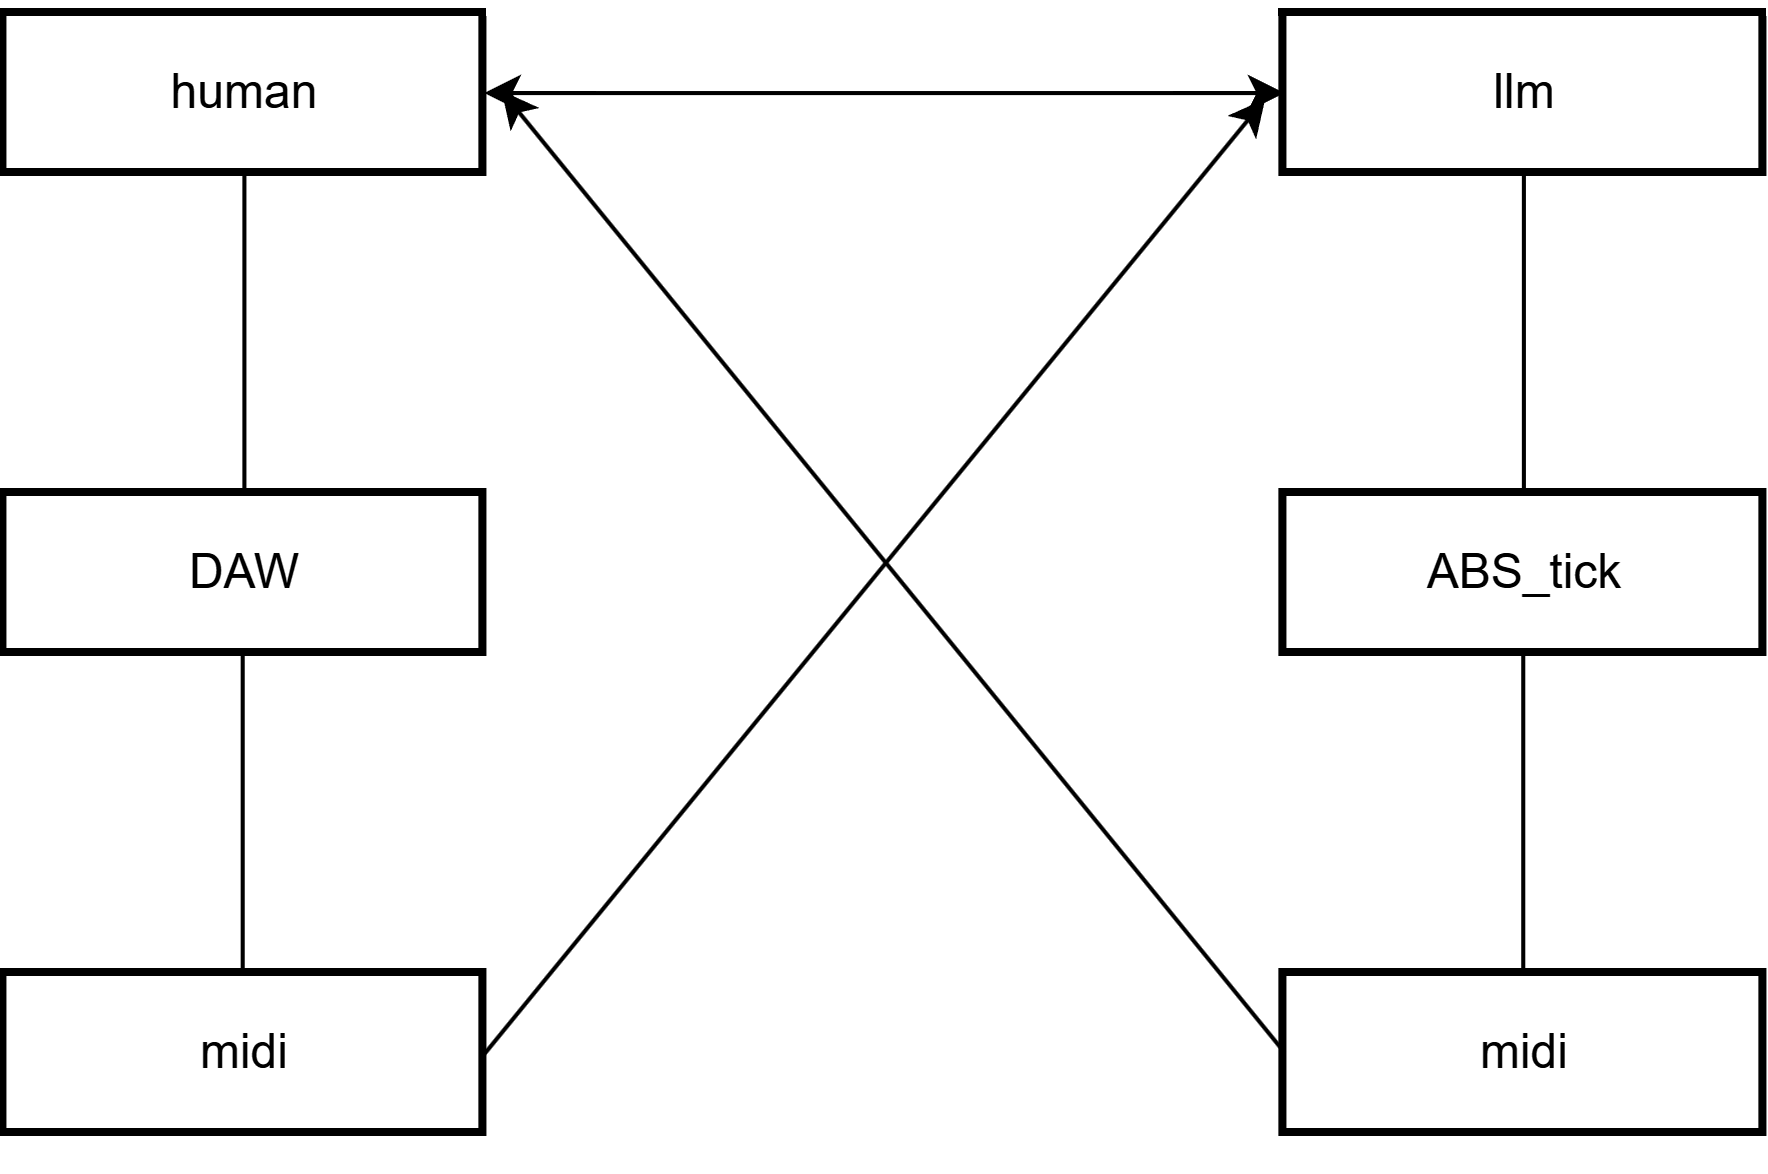
\includegraphics[width=0.54\textwidth]{fig4-hitl.png}
\caption{人机交互路径中的坐标往返。}
\label{fig:hitl}
\end{figure}

\section{讨论}
\label{sec:disc}

\subsection{本工作的性质与定位}

有必要如实说明本工作的性质。核心坐标系的数学本质是\textbf{分段线性函数的
分段求值}，属于平凡内容；唯一的技术点是段内小节索引的相对化 $(M-A_s)$，
并无非平凡的证明。它不产生新的数学知识，而是把一套已知但未经形式化的
工程过程，固化为可调用的规格。

之所以仍值得单独提出，是因为该规格此前\textbf{没有以显式形式存在}：
宿主软件在内部实现了它，却只对外暴露「小节.拍」；把这层映射写成闭式、
给出其退化性质、并明确划出适用边界，是本文所做的工作。
因此准确的说法是：本坐标系不是数学发现，而是一个边界明确的 $O(1)$
计算接口，其价值上限由拍号变化密度决定（第 \ref{sec:domain} 节）。

\subsection{与既有表示体系的关系}

本文的坐标系并不取代 MIDI 消息流或记谱描述语言，而是补足二者之间的映射层。
MIDI 以演奏事件为记录单位，MusicXML 以乐谱版面为描述对象，二者均未提供
一个与拍号无关的绝对位置量；本文所定义的绝对 Tick 正是该缺失量。

\subsection{对音乐理论表述的潜在影响}

本文并不主张用数值取代描述，但指出一处实际变化：若干长期只能以定性方式表达的
概念，在坐标化之后获得了\textbf{可逐对统计}的形式——交叠量、音高差、间隙量
（第 \ref{sec:relation} 节）。这些量在既有表述中依赖「这里连一点」
「这里空一点」这类整体印象，而整体印象难以比较、难以复现。获得定量形式之后，
它们至少可以被比较、被复现、被局部修改。

\subsection{局限}

本文的实验规模有限，结论受以下条件约束。

\begin{enumerate}[leftmargin=2.2em,itemsep=0.15em,topsep=0.2em]
  \item 仅在单一宿主软件上完成校验，尚未与其他实现交叉验证。
  \item 变拍号情形下的取整误差上界尚未给出严格证明，仅有实验观测
        （第 \ref{sec:counter} 节）。
  \item 声部分离中「等距排除法」在三声部以上同时交叉时的正确性尚未证明。
  \item 语义封装层在真实教学场景中的有效性未经用户研究验证。
  \item 第 \ref{sec:case} 节的协同案例为单例观察，无对照组，亦无独立评分者，
        其结论应视为案例证据而非普适主张。
  \item 第 \ref{sec:gen} 节生成架构的两个算例只验证形式约束的一致性，
        未做听感评估，不构成对音乐性的任何主张。
\end{enumerate}

\subsection{未来工作}

以下问题方向明确但本文未及解决，按优先级排列。

\begin{enumerate}[leftmargin=2.2em,itemsep=0.15em,topsep=0.2em]
  \item 给出变拍号取整误差的上界，或证明在特定 PPQ 取值下误差恒为零。
  \item 将等距排除法推广到多声部同时交叉的情形，或刻画其失效条件。
  \item 在第二种宿主软件上复现全部实验，检验结论的实现无关性。
  \item 设计带对照组的听感实验，评估所提生成架构的实际音乐效果。
\end{enumerate}

\section{结论}
本文从宿主软件的界面观察出发，构建了绝对时间坐标系 MATCS，
主要结论为：

\begin{enumerate}[leftmargin=2.2em,itemsep=0.15em,topsep=0.2em]
  \item 音乐事件的位置可被翻译为与拍号、速度、调性无关的绝对 tick 值，
        其形式由式 \eqref{eq:abs} 给出；
  \item 「混合拍子」与「变拍子」在 tick 数学上性质不同，后者才是原式失效的
        真正原因；变拍号条件下原式须推广为分段求和形式 \eqref{eq:master}，
        原式为其 $n=1$ 时的退化特例；
  \item 以「纵向值发生改变的瞬间」为唯一判据，并把休止重新定义为空事件，
        音符与休止的定位逻辑得以统一，时间轴上不再存在未定义区间；
  \item 该形式的适用域受拍号变化密度约束：参数量线性增长，
        密度趋近每小节一变时须切换为拍号事件表加二分查找；
  \item 反向映射不可由人工计算替代，这是该形式真正不可替代之处。
\end{enumerate}

如实地说，本文的数学内容并不厚重：其本质是分段线性函数的分段求值，
唯一的技术点在于段内小节索引的相对化 $(M-A_s)$，并无非平凡的证明。
它的贡献在于把一套已知但未经形式化的工程过程固化为规格，
并明确划出其适用边界。




\appendix

\section{研究日志摘录}
本附录按时间顺序摘录推导过程中的原始记录，正文的若干判据即由此产生。

\begin{引述}
\textbf{第一天 · 刻度稳定性}。在宿主软件中长时间观察「小节.节拍.tick」读数：
无论修改拍号、改变速度还是拖拽素材，该读数始终不变，永远指向同一绝对位置。
\end{引述}

\begin{引述}
\textbf{第二天 · 形式化尝试}。取得式 \eqref{eq:abs} 的雏形，
并以 $4/4$ 拍下第二、第三小节首拍代入验算，得 $3840$ 与 $7680$，
与软件读数一致。
\end{引述}

\begin{引述}
\textbf{第三天 · 反例}。将拍号由 $4/4$ 改为 $6/8$ 后结果出现显著偏差，
拖拽素材或大幅移动音符同样失效。检查偏差数据发现，两种拍号之间存在一个
\textbf{确定的}误差值——误差确定而非随机，说明模型并非错误，而是缺少一个变量。
\end{引述}

\begin{引述}
\textbf{第三天 · 关键观察}。$4/4$ 拍下的八分音符在读数中跨度为 \texttt{0.0.50}，
而 $6/8$ 拍下同样的八分音符读数为 \texttt{0.1.00}。二者 tick 长度相同（$480$），
但被解释为不同的拍数。据此得到结论：时值刻度并非全局常量，
而是由拍号分母决定的局部变量。
\end{引述}

\begin{引述}
\textbf{第四天 · 全局定位}。将 DAW 网格视作平面直角坐标系：横轴已由绝对 Tick
给出，纵轴尚待建立。纵轴的难点不在标记，而在判据——如何判定一个音的开始与结束。
由此得到「事件 $=$ 纵向值发生改变的瞬间」。
\end{引述}

\begin{引述}
\textbf{第五天 · 自我定位}。回顾该形式本身：其数学本质是分段线性函数的分段
求值，属于平凡内容；唯一技术点是段内小节索引的相对化；并无非平凡证明。
它的价值不在于产生新知识，而在于把已知过程固化为可调用的规格。
\end{引述}

\section{核心算法实现}
分段轴构建与双向映射（原实现为 Lua，此处转写为等价形式）：

\begin{museCode}[language=Python]
def build_axis(sections, ppq):
    """sections: [(upToBar, bpi, denom), ...]，upToBar 严格递增"""
    axis, acc_bar, acc_tick = [], 0, 0
    for up_to, bpi, denom in sections:
        bars = up_to - acc_bar
        tpb = round(ppq * 4 / denom)
        axis.append(dict(from_bar=acc_bar + 1, to_bar=up_to, bars=bars,
                         bpi=bpi, tpb=tpb, start_tick=acc_tick,
                         ticks_per_bar=bpi * tpb))
        acc_bar = up_to
        acc_tick += bars * bpi * tpb
    return axis

def pos_to_tick(axis, bar, beat):
    for seg in axis:
        if bar <= seg["to_bar"]:
            rel = bar - seg["from_bar"]
            return seg["start_tick"] + (rel * seg["bpi"] + (beat - 1)) * seg["tpb"]
    raise ValueError("bar 超出轴范围")

def tick_to_pos(axis, tick):
    for i, seg in enumerate(axis):
        seg_end = seg["start_tick"] + seg["bars"] * seg["ticks_per_bar"]
        if tick < seg_end or i == len(axis) - 1:
            local = tick - seg["start_tick"]
            bar_off = local // seg["ticks_per_bar"]
            rem = local - bar_off * seg["ticks_per_bar"]
            beat = rem // seg["tpb"] + 1
            return seg["from_bar"] + bar_off, beat
    raise ValueError("tick 超出轴范围")
\end{museCode}

\section{术语表}
\begin{longtable}{@{}p{3.4cm}p{11.1cm}@{}}
\caption{核心术语}\label{tab:glossary}\\
\toprule
\thd{术语} & \thd{含义} \\
\midrule
\endfirsthead
\multicolumn{2}{@{}l}{\small\itshape （续）}\\
\toprule
\thd{术语} & \thd{含义} \\
\midrule
\endhead
\bottomrule
\endlastfoot
MATCS & Mozun Absolute Time Coordinate System，本文提出的绝对时间坐标系 \\
绝对 Tick & 自工程起点至该事件的 tick 计数，与拍号、速度、调性无关 \\
空事件 & 音高属性为空、具有明确起止时刻的事件；休止即其一例 \\
事件链 & 相邻事件终点与起点首尾相接构成的不间断序列 \\
TPB & 每拍数值坐标单位数，$=\mathrm{PPQ}\times 4/\mathrm{Denom}$ \\
BPI & Beats Per Bar，每小节拍数，等于拍号分子 \\
PPQ & Pulses Per Quarter Note，系统预设时间分辨率 \\
Denom & 拍号分母，决定「一拍」对应何种音符 \\
单拍子 & $2/4$、$3/4$ 等，单一重音组 \\
复拍子 & $6/8$、$9/8$、$12/8$，每「拍」为附点音符 \\
混合拍子 & $5/8$、$7/8$，小节内不等分，拍号本身不变 \\
\textbf{变拍子} & 作品中途更换拍号，须分段处理 \\
段表 & 记录各拍号段 $n_k,p_k,d_k$ 的前置元数据 \\
段起点 $S_s$ & 第 $s$ 段起始处的累计 tick 边界 \\
锚点 & 测量相对距离时选定的参照位置 \\
纵向值 & 某绝对 tick 上的音高状态，$0$ 表示休止 \\
tick\_translate & 位置表示与绝对坐标之间的双向映射引擎 \\
line\_for\_llm & 面向语言模型的结构化语义封装层 \\
\end{longtable}

\end{document}

\end{document}
